\subsection{Systematic Uncertainties}\label{sec:WBoson_Analysis_Systematics}

This section presents the different sources and the procedure used to determine the systematic uncertainties in the measurement of the \W forward-backward ratios, the muon charge asymmetry and the \W cross sections.

%%------------------------------------------------------------%%
\subsubsection{Luminosity}

The integrated luminosity of the 2016 \pPb data sample processed is $173.4 \pm 5\%$~\nbinv as presented in \sect{sec:WBoson_Analysis_DataSamples}. Since the integrated luminosity cancels in the forward-backward ratios and charge asymmetry, it only affects the measurement of the \WToMuNu differential cross sections. In this case, the systematic uncertainty is taken as a global uncertainty of $5\%$ and the bin-to-bin correlation is +100\%.

%%------------------------------------------------------------%%
\subsubsection{Muon Efficiency}

\subsubsection{MC Statistics}

A systematic uncertainty is assigned to account for the limited statistics in the MC samples used to compute the muon efficiency. The MC statistical uncertainty of the muon efficiencies is determined as explained in \sect{sec:WBoson_Analysis_MCTruthEfficiency} and then propagated to all the observables. The uncertainty is considered to be fully uncorrelated. The systematic uncertainty on each observable due to the MC statistics is shown in \fig{fig:Systematic_Eff_MC_Statistics}.

\begin{figure}[!htbp]
 \begin{center}
  \includegraphics[width=0.30\textwidth]{Figures/WBoson/Analysis/Systematics/Variation/PA/Cross_Section/gr_WToMuMi_PA_Cross_Section_EffTnP_MC_Statistics.pdf}
  \includegraphics[width=0.30\textwidth]{Figures/WBoson/Analysis/Systematics/Variation/PA/ForwardBackward_Ratio/gr_WToMuMi_PA_ForwardBackward_Ratio_EffTnP_MC_Statistics.pdf}
  \includegraphics[width=0.30\textwidth]{Figures/WBoson/Analysis/Systematics/Variation/PA/ForwardBackward_Ratio/gr_WToMuInc_PA_ForwardBackward_Ratio_EffTnP_MC_Statistics.pdf}
%%
  \includegraphics[width=0.30\textwidth]{Figures/WBoson/Analysis/Systematics/Variation/PA/Cross_Section/gr_WToMuPl_PA_Cross_Section_EffTnP_MC_Statistics.pdf}
  \includegraphics[width=0.30\textwidth]{Figures/WBoson/Analysis/Systematics/Variation/PA/ForwardBackward_Ratio/gr_WToMuPl_PA_ForwardBackward_Ratio_EffTnP_MC_Statistics.pdf}
  \includegraphics[width=0.30\textwidth]{Figures/WBoson/Analysis/Systematics/Variation/PA/Charge_Asymmetry/gr_WToMuInc_PA_Charge_Asymmetry_EffTnP_MC_Statistics.pdf}
 \end{center}
 \caption{Systematic uncertainty due to the MC statistical error of the corrected efficiency. The plots are divided as: \WToMuNuMi (top-left) and \WToMuNuPl (bottom-left) cross sections, $\W^{-}$ (top-middle) and $\W^{+}$ (bottom-middle) $R_{FB}$, and finally the \W $R_{FB}$ (top-right) and \W charge asymmetry (bottom-right). The values between square parenthesis represents the maximum and minimum relative uncertainty for the case of the cross sections and the absolute uncertainty for the $R_{FB}$ and charge asymmetry.}
 \label{fig:Systematic_Eff_MC_Statistics}
\end{figure}

\subsubsection{Theory Model}

The NLO model used to generate the MC \POWHEG samples can impact the measurement of the muon efficiencies. The main sources of theory uncertainties include the choice of the nuclear parton distribution function (EPPS16+CT14), renormalization scale, factorization scale and $\alpha_{s}$. The theory uncertainties are assumed to be correlated in both charge and $\eta_{CM}$.

Since the PDFs are not calculable from first principles but are determined experimentally, the inclusion of any PDF introduces an additional systematic error. Therefore, a study is performed to estimate the effect of a PDF change in the \POWHEG generator on the muon efficiencies.

The procedure used to derive the theory uncertainties of the PDF variations consist of reweighting the MC events using the weights produced by \POWHEG after applying each PDF set. The PDF sets are accessed through the LHAPDF v6 \cite{LHAPDF6} framework and consist of 56 CT14 PDFs, 40 EPPS16 nuclear corrections and 2 CT14 $\alpha_{s}$ variations. Once the MC samples are reweighted with each PDF set, the efficiencies are recomputed and used to recalculate all the observables.

The nPDF uncertainty is determined by combining the EPPS16+CT14 variations of the observables using the Hessian approach as recommended by the EPPS16 authors (see Eq.~29 of Ref.~\cite{EPS09}). The EPPS16+CT14 sets corresponds to 90$\%$ confidence interval (CL) variations, so the uncertainties are scaled to 68$\%$. The results of the nPDF systematic uncertainty are shown in \fig{fig:Systematic_MC_Syst_PDF}.

\begin{figure}[!htbp]
 \begin{center}
  \includegraphics[width=0.30\textwidth]{Figures/WBoson/Analysis/Systematics/PDF/PA/Cross_Section/gr_WToMuMi_PA_Cross_Section_EffTnP_MC_Syst_PDF.pdf}
  \includegraphics[width=0.30\textwidth]{Figures/WBoson/Analysis/Systematics/PDF/PA/ForwardBackward_Ratio/gr_WToMuMi_PA_ForwardBackward_Ratio_EffTnP_MC_Syst_PDF.pdf}
  \includegraphics[width=0.30\textwidth]{Figures/WBoson/Analysis/Systematics/PDF/PA/ForwardBackward_Ratio/gr_WToMuInc_PA_ForwardBackward_Ratio_EffTnP_MC_Syst_PDF.pdf}
%%
  \includegraphics[width=0.30\textwidth]{Figures/WBoson/Analysis/Systematics/PDF/PA/Cross_Section/gr_WToMuPl_PA_Cross_Section_EffTnP_MC_Syst_PDF.pdf}
  \includegraphics[width=0.30\textwidth]{Figures/WBoson/Analysis/Systematics/PDF/PA/ForwardBackward_Ratio/gr_WToMuPl_PA_ForwardBackward_Ratio_EffTnP_MC_Syst_PDF.pdf}
  \includegraphics[width=0.30\textwidth]{Figures/WBoson/Analysis/Systematics/PDF/PA/Charge_Asymmetry/gr_WToMuInc_PA_Charge_Asymmetry_EffTnP_MC_Syst_PDF.pdf}
 \end{center}
 \caption{Systematic uncertainty corresponding to the EPPS16+CT14 nPDF variations. The plots are divided as: \WToMuNuMi (top-left) and \WToMuNuPl (bottom-left) cross sections, $\W^{-}$ (top-middle) and $\W^{+}$ (bottom-middle) $R_{FB}$, and finally the \W $R_{FB}$ (top-right) and \W charge asymmetry (bottom-right). The values between square parenthesis represents the maximum and minimum relative uncertainty for the case of the cross sections and the absolute uncertainty for the $R_{FB}$ and charge asymmetry. The red lines represent each of the 96 nPDF variations. }
 \label{fig:Systematic_MC_Syst_PDF}
\end{figure}


\clearpage
Furthermore, the $\alpha_{s}$ uncertainty is determined by using the EPPS16+CT14 nPDFs associated to the $\alpha_{s}\left(m_{Z}^{2}\right)$ values: 0.1170 and 0.1190. The variations on the observables are combined following the prescription recommended in the PDF4LHC15~\cite{PDF4LHC}, which basically corresponds to taking the average per bin of the two variations. The uncertainties are converted to 68$\%$ CL after rescaling them by $0.0015/0.0010$ as described in PDF4LHC15~\cite{PDF4LHC}. The results of the $\alpha_{s}$ systematic uncertainty are shown in \fig{fig:Systematic_MC_Syst_Alpha}.

\begin{figure}[!htbp]
 \begin{center}
  \includegraphics[width=0.30\textwidth]{Figures/WBoson/Analysis/Systematics/PDF/PA/Cross_Section/gr_WToMuMi_PA_Cross_Section_EffTnP_MC_Syst_Alpha.pdf}
  \includegraphics[width=0.30\textwidth]{Figures/WBoson/Analysis/Systematics/PDF/PA/ForwardBackward_Ratio/gr_WToMuMi_PA_ForwardBackward_Ratio_EffTnP_MC_Syst_Alpha.pdf}
  \includegraphics[width=0.30\textwidth]{Figures/WBoson/Analysis/Systematics/PDF/PA/ForwardBackward_Ratio/gr_WToMuInc_PA_ForwardBackward_Ratio_EffTnP_MC_Syst_Alpha.pdf}
%%
  \includegraphics[width=0.30\textwidth]{Figures/WBoson/Analysis/Systematics/PDF/PA/Cross_Section/gr_WToMuPl_PA_Cross_Section_EffTnP_MC_Syst_Alpha.pdf}
  \includegraphics[width=0.30\textwidth]{Figures/WBoson/Analysis/Systematics/PDF/PA/ForwardBackward_Ratio/gr_WToMuPl_PA_ForwardBackward_Ratio_EffTnP_MC_Syst_Alpha.pdf}
  \includegraphics[width=0.30\textwidth]{Figures/WBoson/Analysis/Systematics/PDF/PA/Charge_Asymmetry/gr_WToMuInc_PA_Charge_Asymmetry_EffTnP_MC_Syst_Alpha.pdf}
 \end{center}
 \caption{Systematic uncertainty corresponding to the $\alpha_{s}$ variations. The plots are divided as: \WToMuNuMi (top-left) and \WToMuNuPl (bottom-left) cross sections, $\W^{-}$ (top-middle) and $\W^{+}$ (bottom-middle) $R_{FB}$, and finally the \W $R_{FB}$ (top-right) and \W charge asymmetry (bottom-right). The values between square parenthesis represents the maximum and minimum relative uncertainty for the case of the cross sections and the absolute uncertainty for the $R_{FB}$ and charge asymmetry. The red and blue lines represent the up and down variations of $\alpha_{s}$, respectively.}
 \label{fig:Systematic_MC_Syst_Alpha}
\end{figure}


And finally, the uncertainty due to the renormalization ($\mu_{R}$) and factorization ($\mu_{F}$) scales, is computed by varying the two scales in \POWHEG using the following sets:

\begin{equation*}
(\mu_{R} , \mu_{F}) = [\ (0.5 , 0.5)\ ,\ (1.0 , 0.5)\ ,\ (0.5 , 1.0)\ ,\ (1.0 , 2.0)\ ,\ (2.0 , 1.0)\ ,\ (2.0 , 2.0)\ ]
\end{equation*}

The MC samples are reweighted event by event using the \POWHEG weights produced with each set of scales, then the efficiencies are recomputed and the observables are recalculated for each varied efficiency. The variations on the observables are combined by taking the envelope (i.e. the maximum variation in each $\eta_{CM}$ bin). The uncertainties are considered 68$\%$ CL. The systematic uncertainties due to the change of $(\mu_{R} , \mu_{F})$ scales are shown in \fig{fig:Systematic_MC_Syst_Scale}.

\begin{figure}[!htbp]
 \begin{center}
  \includegraphics[width=0.30\textwidth]{Figures/WBoson/Analysis/Systematics/PDF/PA/Cross_Section/gr_WToMuMi_PA_Cross_Section_EffTnP_MC_Syst_Scale.pdf}
  \includegraphics[width=0.30\textwidth]{Figures/WBoson/Analysis/Systematics/PDF/PA/ForwardBackward_Ratio/gr_WToMuMi_PA_ForwardBackward_Ratio_EffTnP_MC_Syst_Scale.pdf}
  \includegraphics[width=0.30\textwidth]{Figures/WBoson/Analysis/Systematics/PDF/PA/ForwardBackward_Ratio/gr_WToMuInc_PA_ForwardBackward_Ratio_EffTnP_MC_Syst_Scale.pdf}
%%
  \includegraphics[width=0.30\textwidth]{Figures/WBoson/Analysis/Systematics/PDF/PA/Cross_Section/gr_WToMuPl_PA_Cross_Section_EffTnP_MC_Syst_Scale.pdf}
  \includegraphics[width=0.30\textwidth]{Figures/WBoson/Analysis/Systematics/PDF/PA/ForwardBackward_Ratio/gr_WToMuPl_PA_ForwardBackward_Ratio_EffTnP_MC_Syst_Scale.pdf}
  \includegraphics[width=0.30\textwidth]{Figures/WBoson/Analysis/Systematics/PDF/PA/Charge_Asymmetry/gr_WToMuInc_PA_Charge_Asymmetry_EffTnP_MC_Syst_Scale.pdf}
 \end{center}
 \caption{Systematic variation corresponding to the renormalization and factorization scale variations. The plots are divided as: \WToMuNuMi (top-left) and \WToMuNuPl (bottom-left) cross sections, $\W^{-}$ (top-middle) and $\W^{+}$ (bottom-middle) $R_{FB}$, and finally the \W $R_{FB}$ (top-right) and \W charge asymmetry (bottom-right). The values between square parenthesis represents the maximum and minimum relative uncertainty for the case of the cross sections and the absolute uncertainty for the $R_{FB}$ and charge asymmetry. The red lines represent each of the 6 sets of scale variations. }
 \label{fig:Systematic_MC_Syst_Scale}
\end{figure}

\clearpage
\subsubsection{Tag-and-Probe Correction}

The main source of systematic uncertainty in the measurement of the muon efficiency arises from the application of the TnP scale factors used to correct the truth efficiency. As mentioned in \sect{sec:WBoson_Analysis_CorrectedEfficiency}, the statitstical and systematic uncertainties of the TnP correction is composed by the different components that enters the muon efficiency: trigger, identification, isolation, reconstruction, event activity and pileup.

Since this analysis measures the forward-backward ratios and the charge asymmetry of \W bosons, it is crucial to consider the correlation between the different TnP uncertainties as a function of muon $\eta_{CM}$ and charge. The statistical TnP variations are considered correlated only within the $\eta_{LAB}$ bins (see \cite{Muon_TnP_pPb}) in which they were derived ($\eta_{LAB}$ bin in the case of trigger, $|\eta_{LAB}|$ bin in the case of identification and isolation), while no correlation is assumed with respect to the muon charge. The systematic TnP variations are expected to be fully correlated as a function of muon charge and uncorrelated between the different $\eta_{CM}$. The correlations of each source of TnP uncertainty are listed in \tab{tab:systcorr}.

\begin{table}[!htb]
 \caption{Summary of the correlations per source of tag and probe uncertainty, as a function of muon pseudorapidity (in the laboratory frame) and charge. The $\eta$ (for trigger) or $|\eta|$ (for ID and isolation) ranges are the ones defined in \href{https://github.com/CMS-HIN-dilepton/MuonAnalysis-TagAndProbe/blob/80X_HI/macros/tnp_weight.h}{\underline{the tnp header file}} and mentioned before. When a correlation per $\eta$ or $|\eta|$ range is mentioned, the different ranges are uncorrelated between them.
 \label{tab:systcorr}}
 
 \begin{center}
 \begin{tabular}{l|c|c}
 \hline
 Source of uncertainty & correlation in muon $\eta$ & correlation in muon charge \\
 \hline
 Trigger, stat. & yes per $\eta$ range & no \\
 ID, stat. & yes per $|\eta|$ range & no \\
 Iso, stat. & yes per $|\eta|$ range & no \\
 Trigger, syst. & no & yes \\
 ID, syst. & no & yes \\
 Iso, syst. & no & yes \\
 ID, syst. binned & no & yes \\
 Iso, syst. binned & no & yes \\
 HF$+$PU & no & yes \\
 STA & no & yes \\
 \hline
 \end{tabular}
 \end{center}
\end{table}

To compute the uncertainties, the muon charge asymmetry and the forward-backward ratios are recalculated for each efficiency derived by varying the TnP scale factors. The TnP uncertainties are then determined by taking the difference between the value obtained with the varied TnP SF and its nominal value, combining the uncertainties as explained in \sect{sec:WBoson_Analysis_CorrectedEfficiency}. If the TnP source is correlated in muon charge or pseudorapidity, the corresponding \W yields are varied at the same time. Moreover, for the $\W^{\pm}$ cross sections, the statistical and systematic TnP uncertainties are calculated by propagating the uncertainties on the corrected muon efficiency due to the TnP variations as listed in Appendix~\ref{app:TnPUncertainties}. The results of the TnP systematic and statistical variations are shown in \fig{fig:Systematic_Eff_TnP_Syst} and \fig{fig:Systematic_Eff_TnP_Stat}, respectively.


\begin{figure}[!htbp]
 \begin{center}
  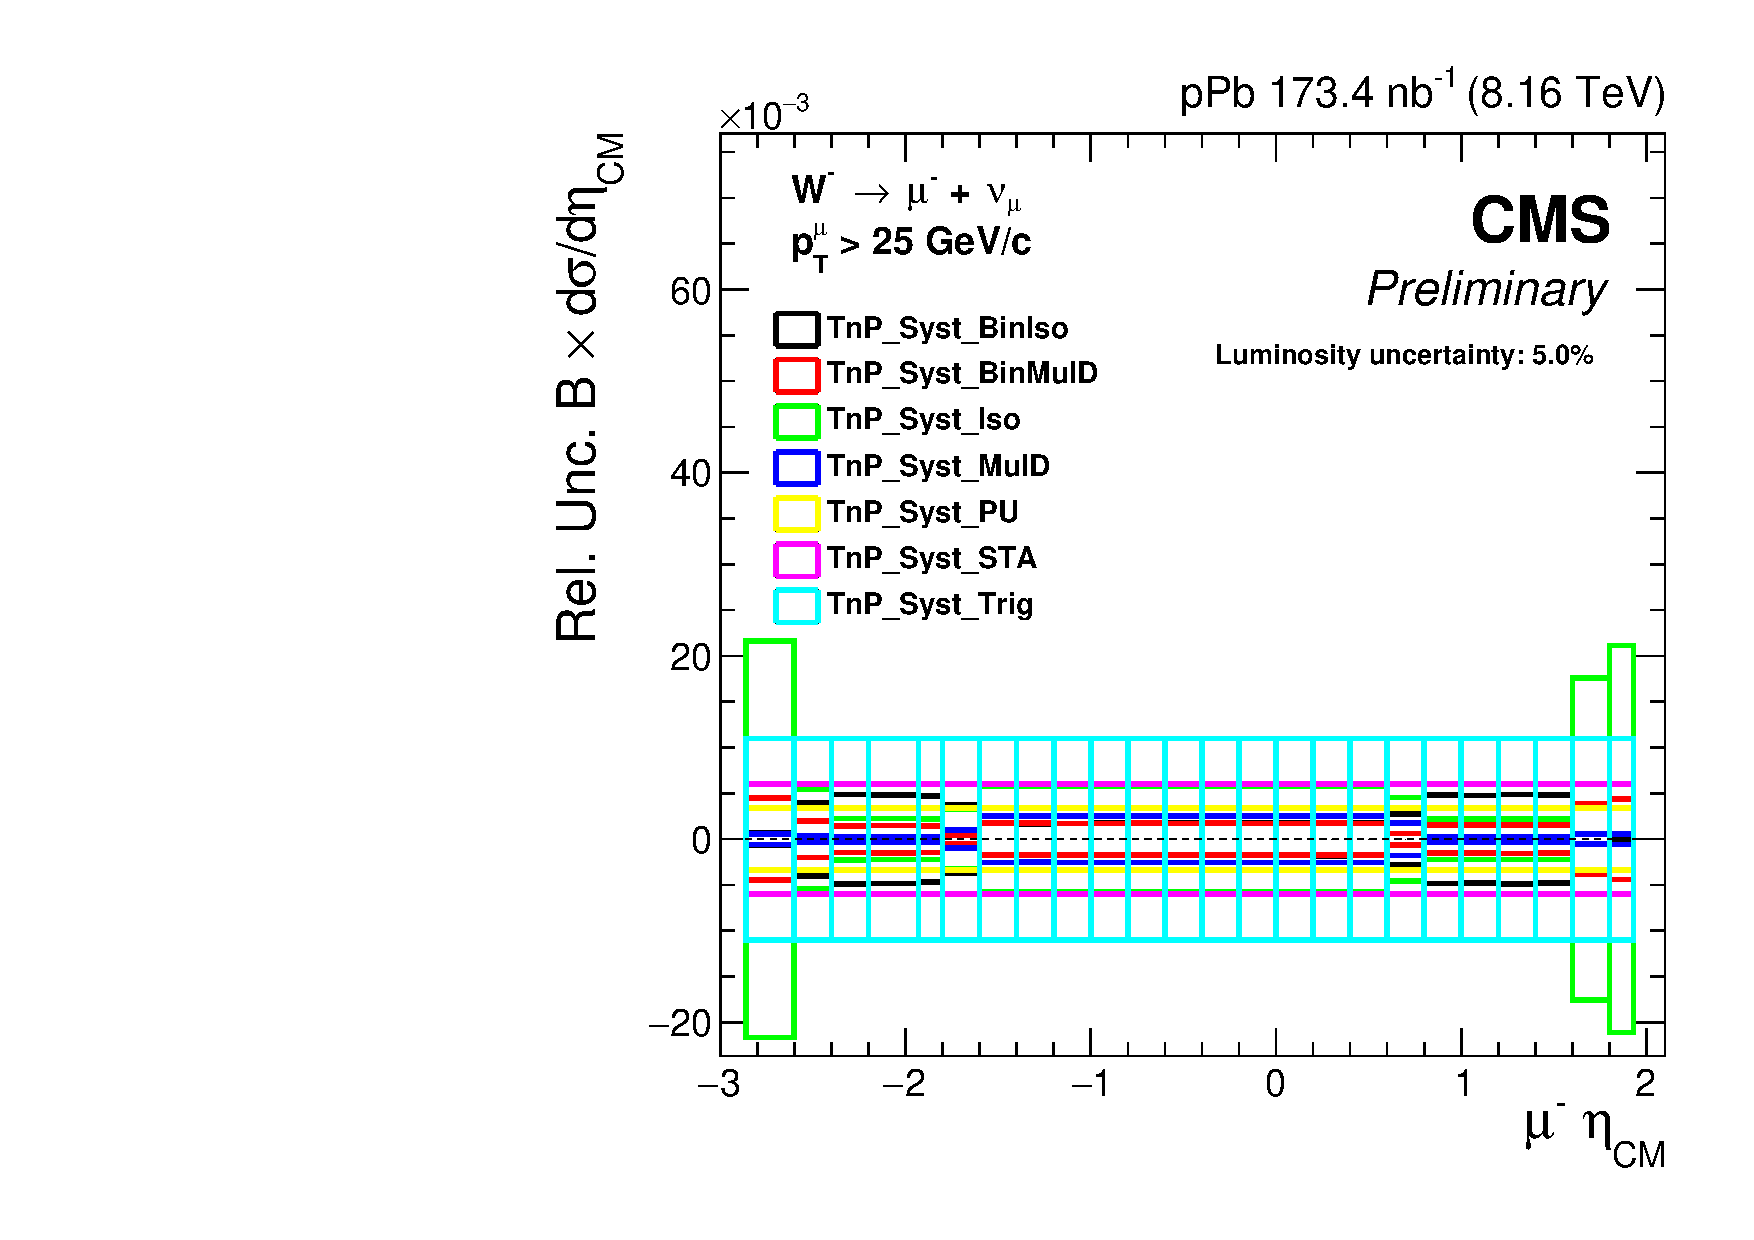
\includegraphics[width=0.29\textwidth]{Figures/WBoson/Analysis/Systematics/Combined/PA/Cross_Section/gr_WToMuMi_PA_Cross_Section_EffTnP_TnP_Syst.pdf}
  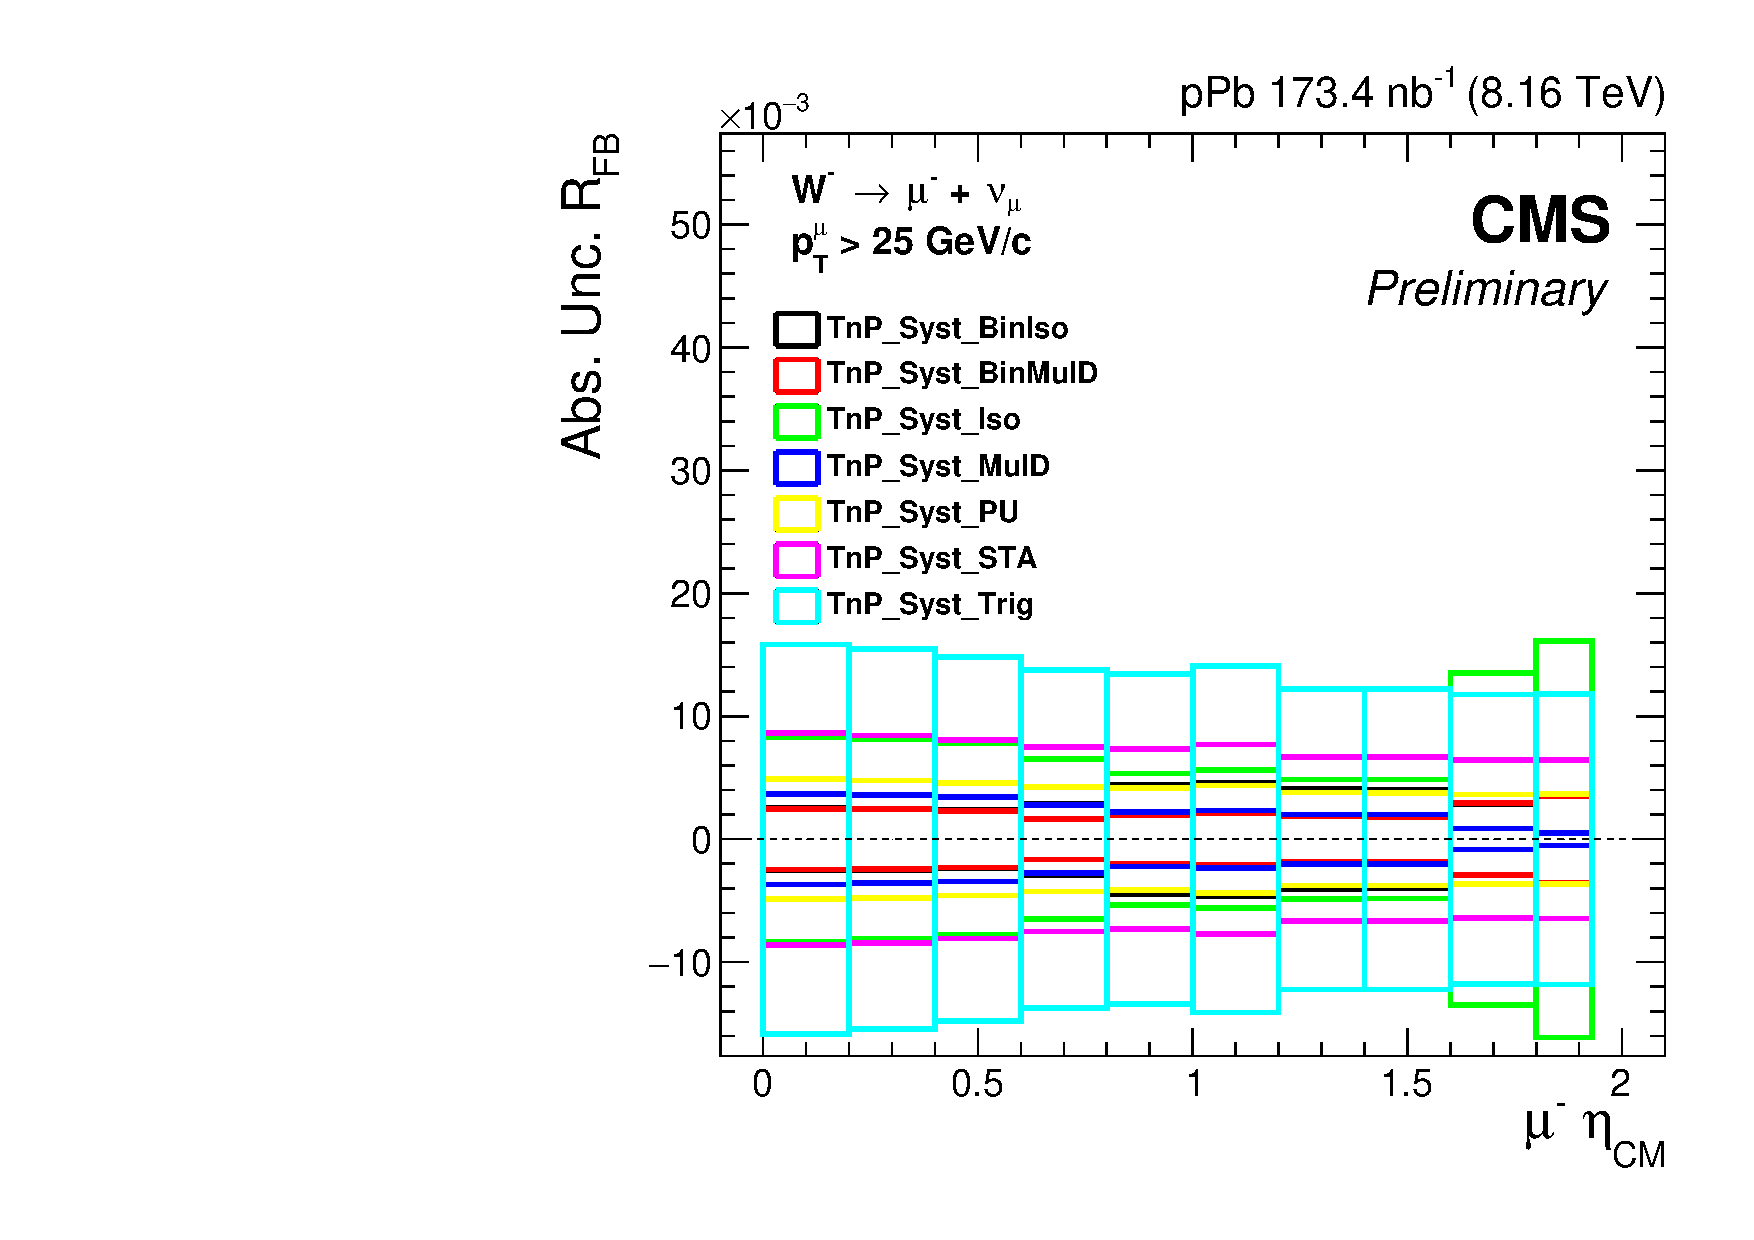
\includegraphics[width=0.29\textwidth]{Figures/WBoson/Analysis/Systematics/Combined/PA/ForwardBackward_Ratio/gr_WToMuMi_PA_ForwardBackward_Ratio_EffTnP_TnP_Syst.pdf}
  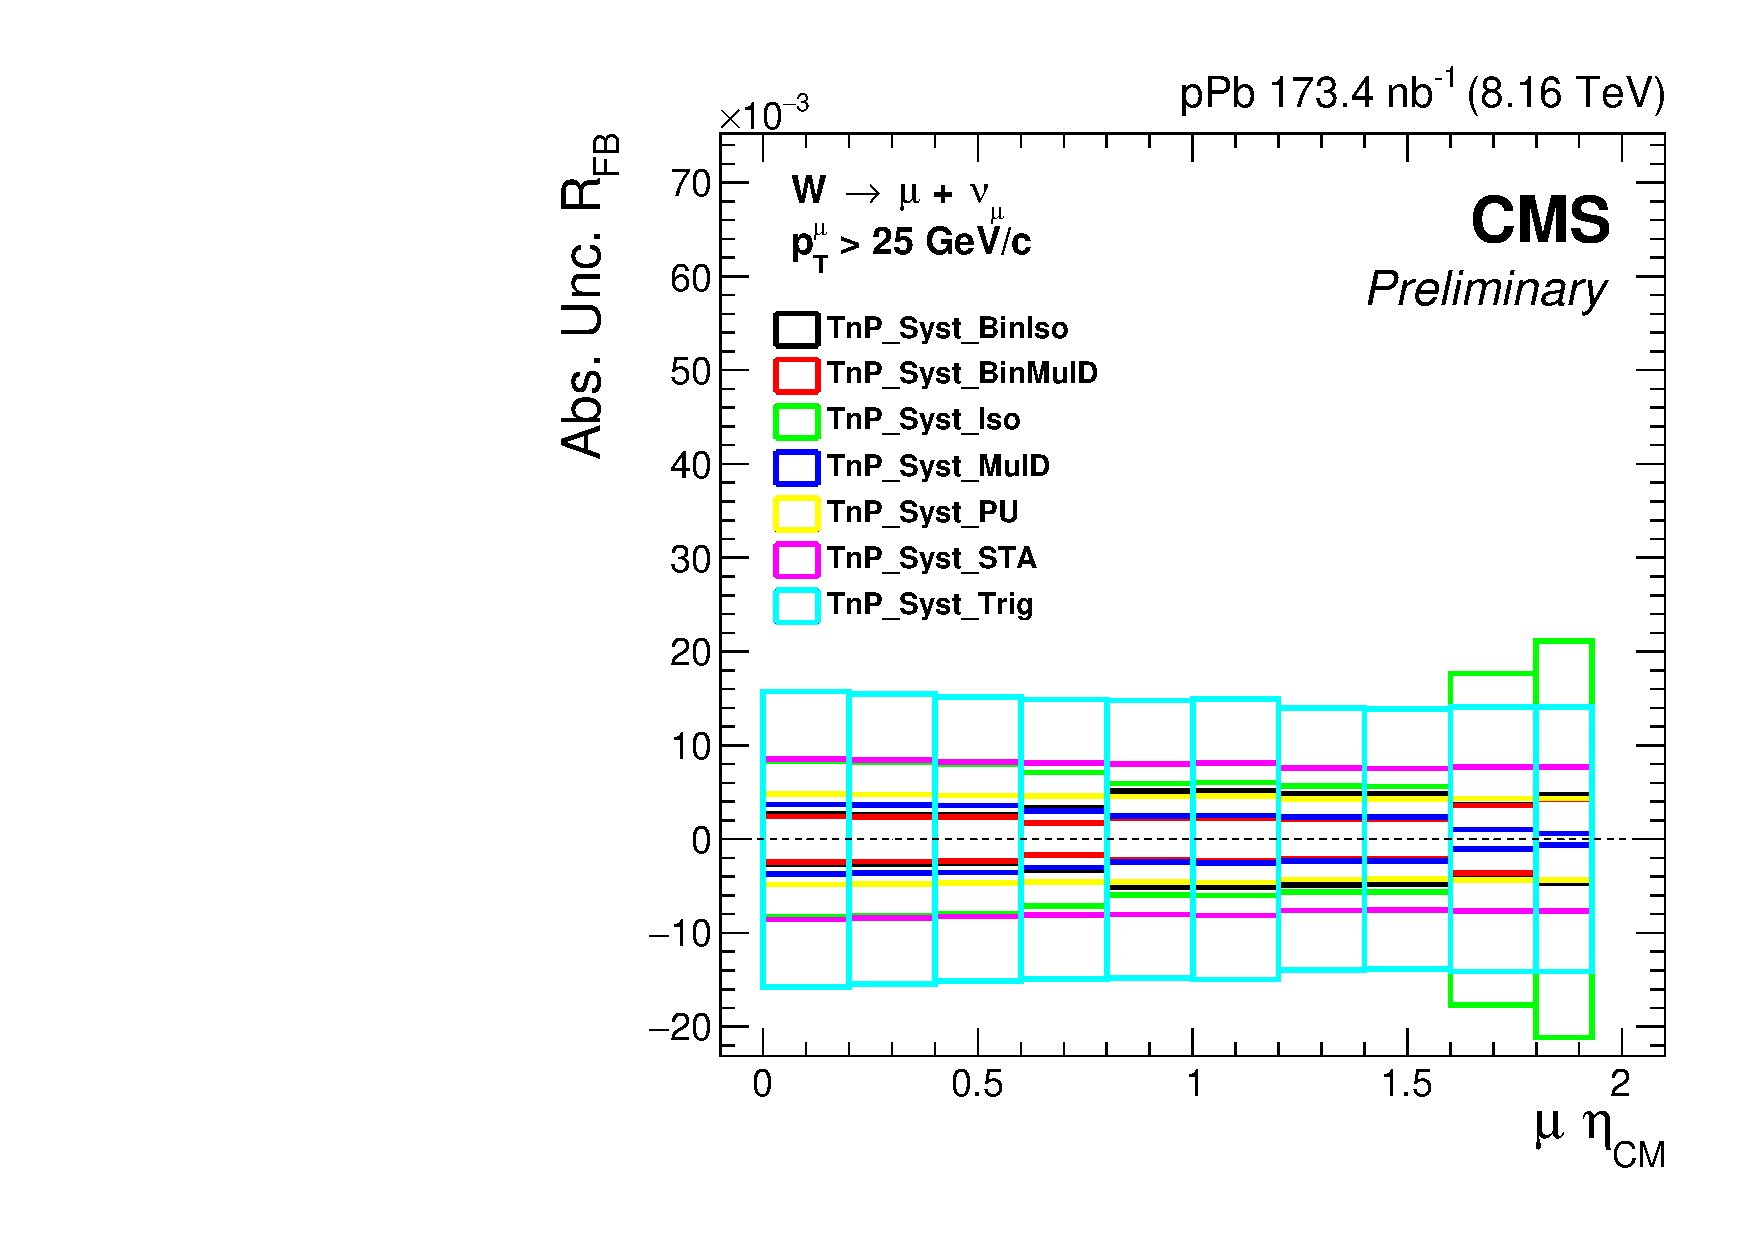
\includegraphics[width=0.29\textwidth]{Figures/WBoson/Analysis/Systematics/Combined/PA/ForwardBackward_Ratio/gr_WToMuInc_PA_ForwardBackward_Ratio_EffTnP_TnP_Syst.pdf}
%%
  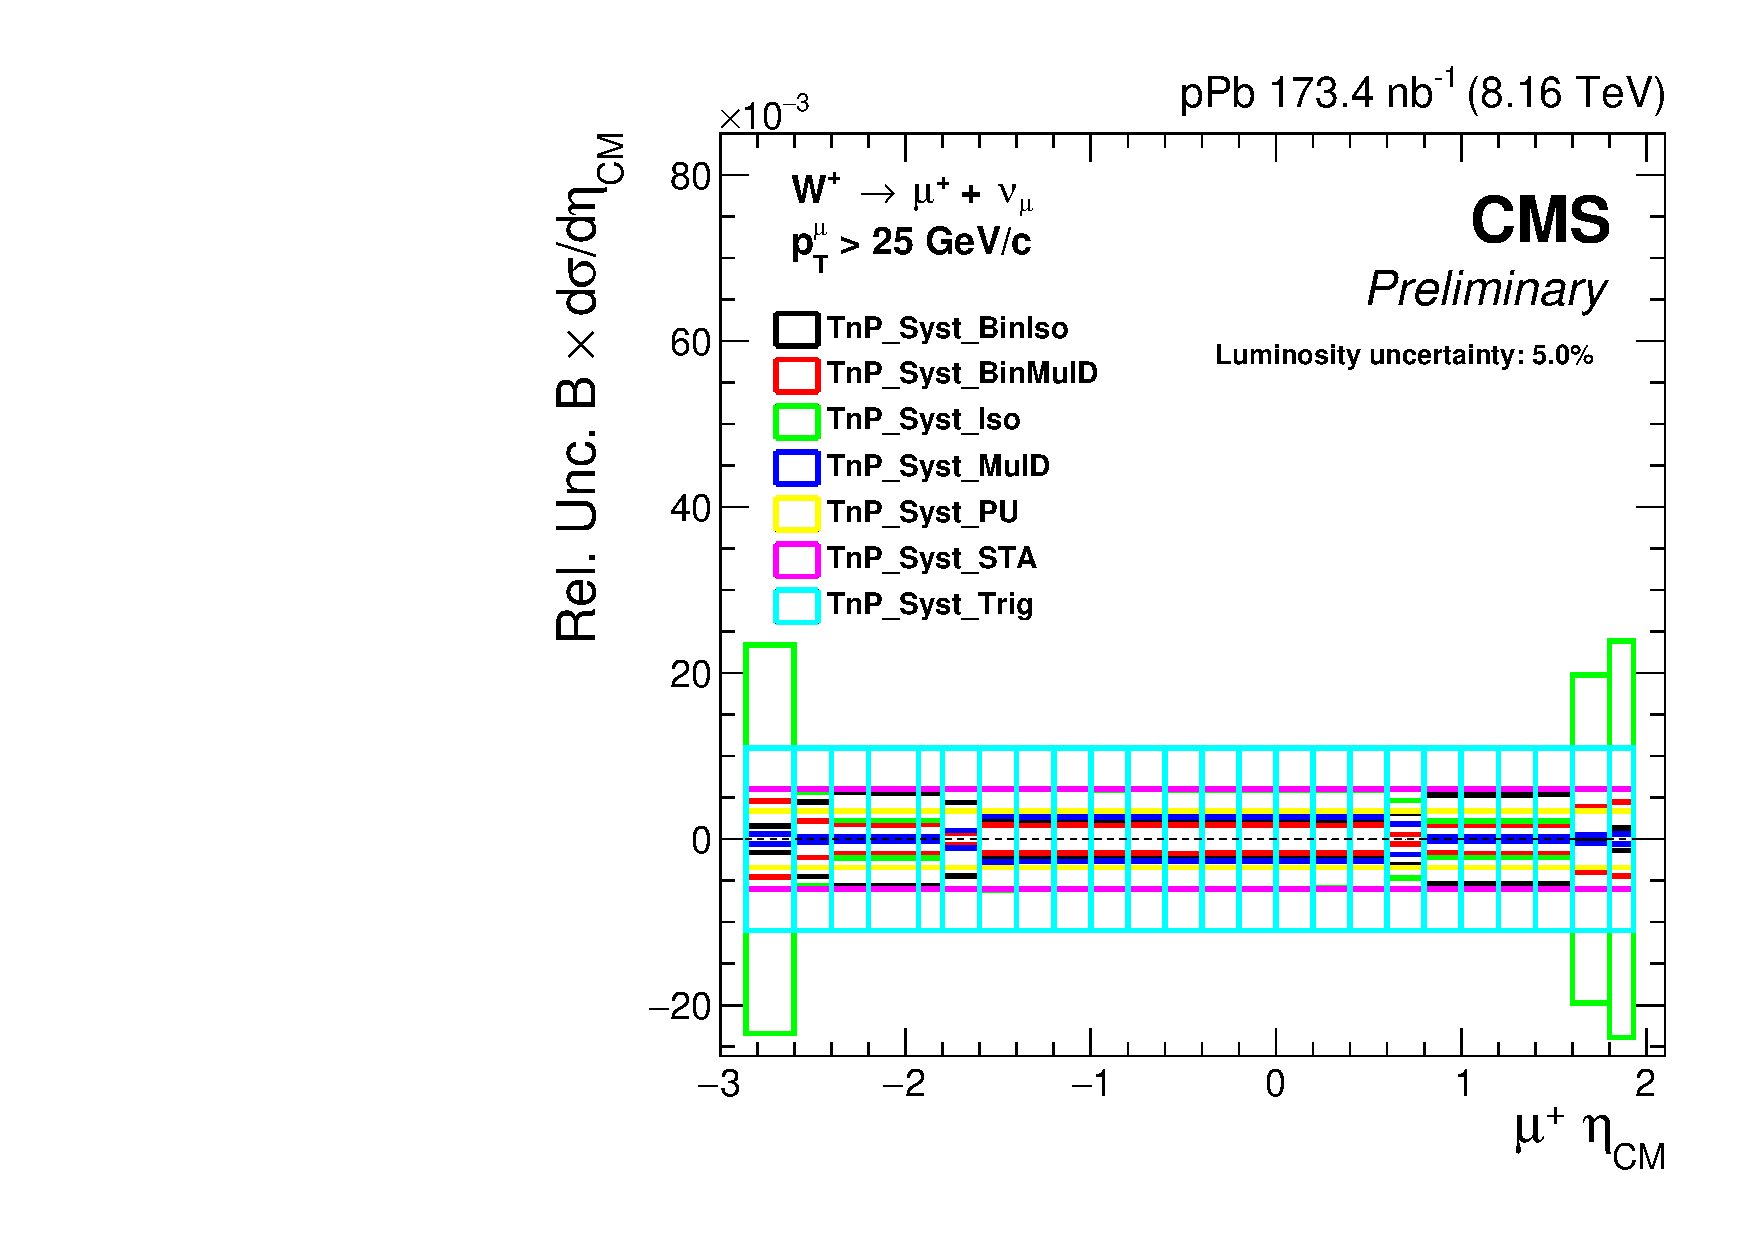
\includegraphics[width=0.29\textwidth]{Figures/WBoson/Analysis/Systematics/Combined/PA/Cross_Section/gr_WToMuPl_PA_Cross_Section_EffTnP_TnP_Syst.pdf}
  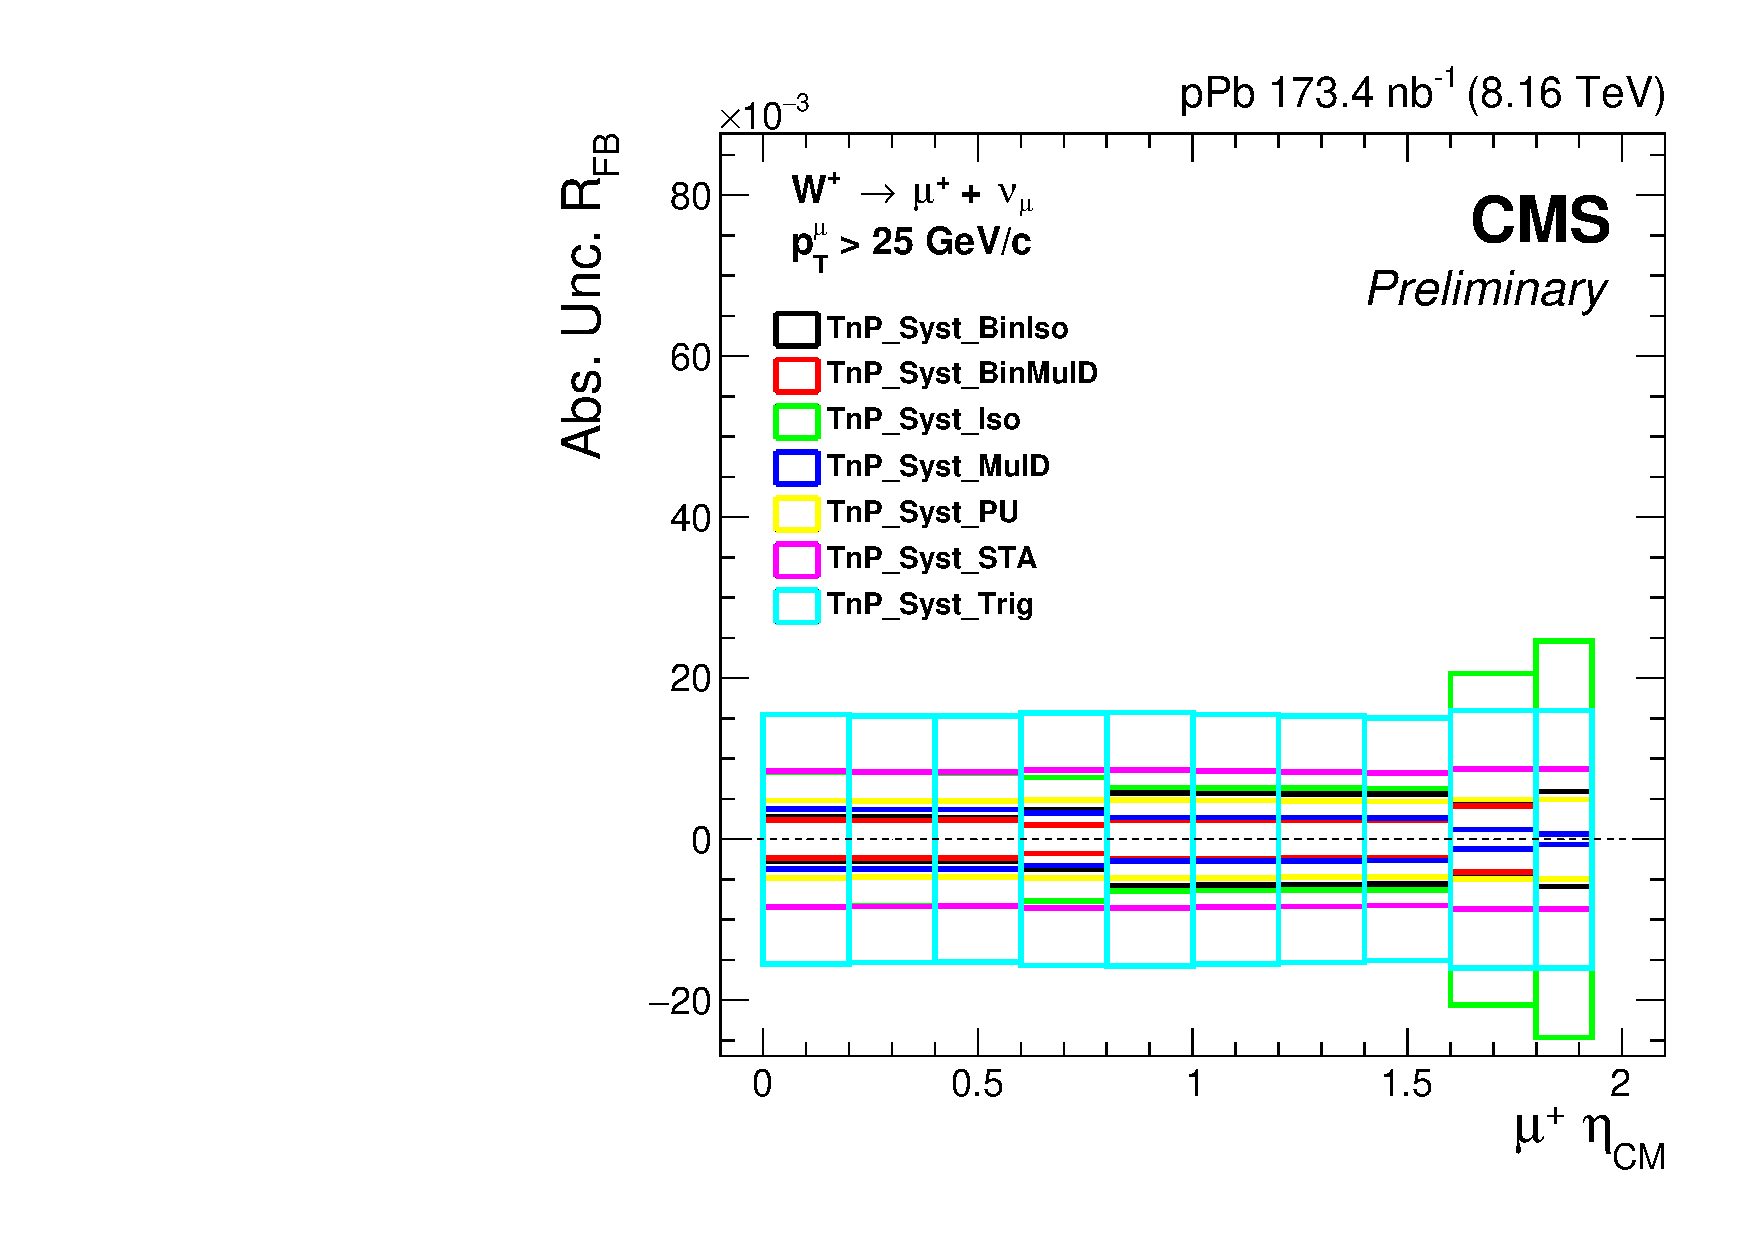
\includegraphics[width=0.29\textwidth]{Figures/WBoson/Analysis/Systematics/Combined/PA/ForwardBackward_Ratio/gr_WToMuPl_PA_ForwardBackward_Ratio_EffTnP_TnP_Syst.pdf}
  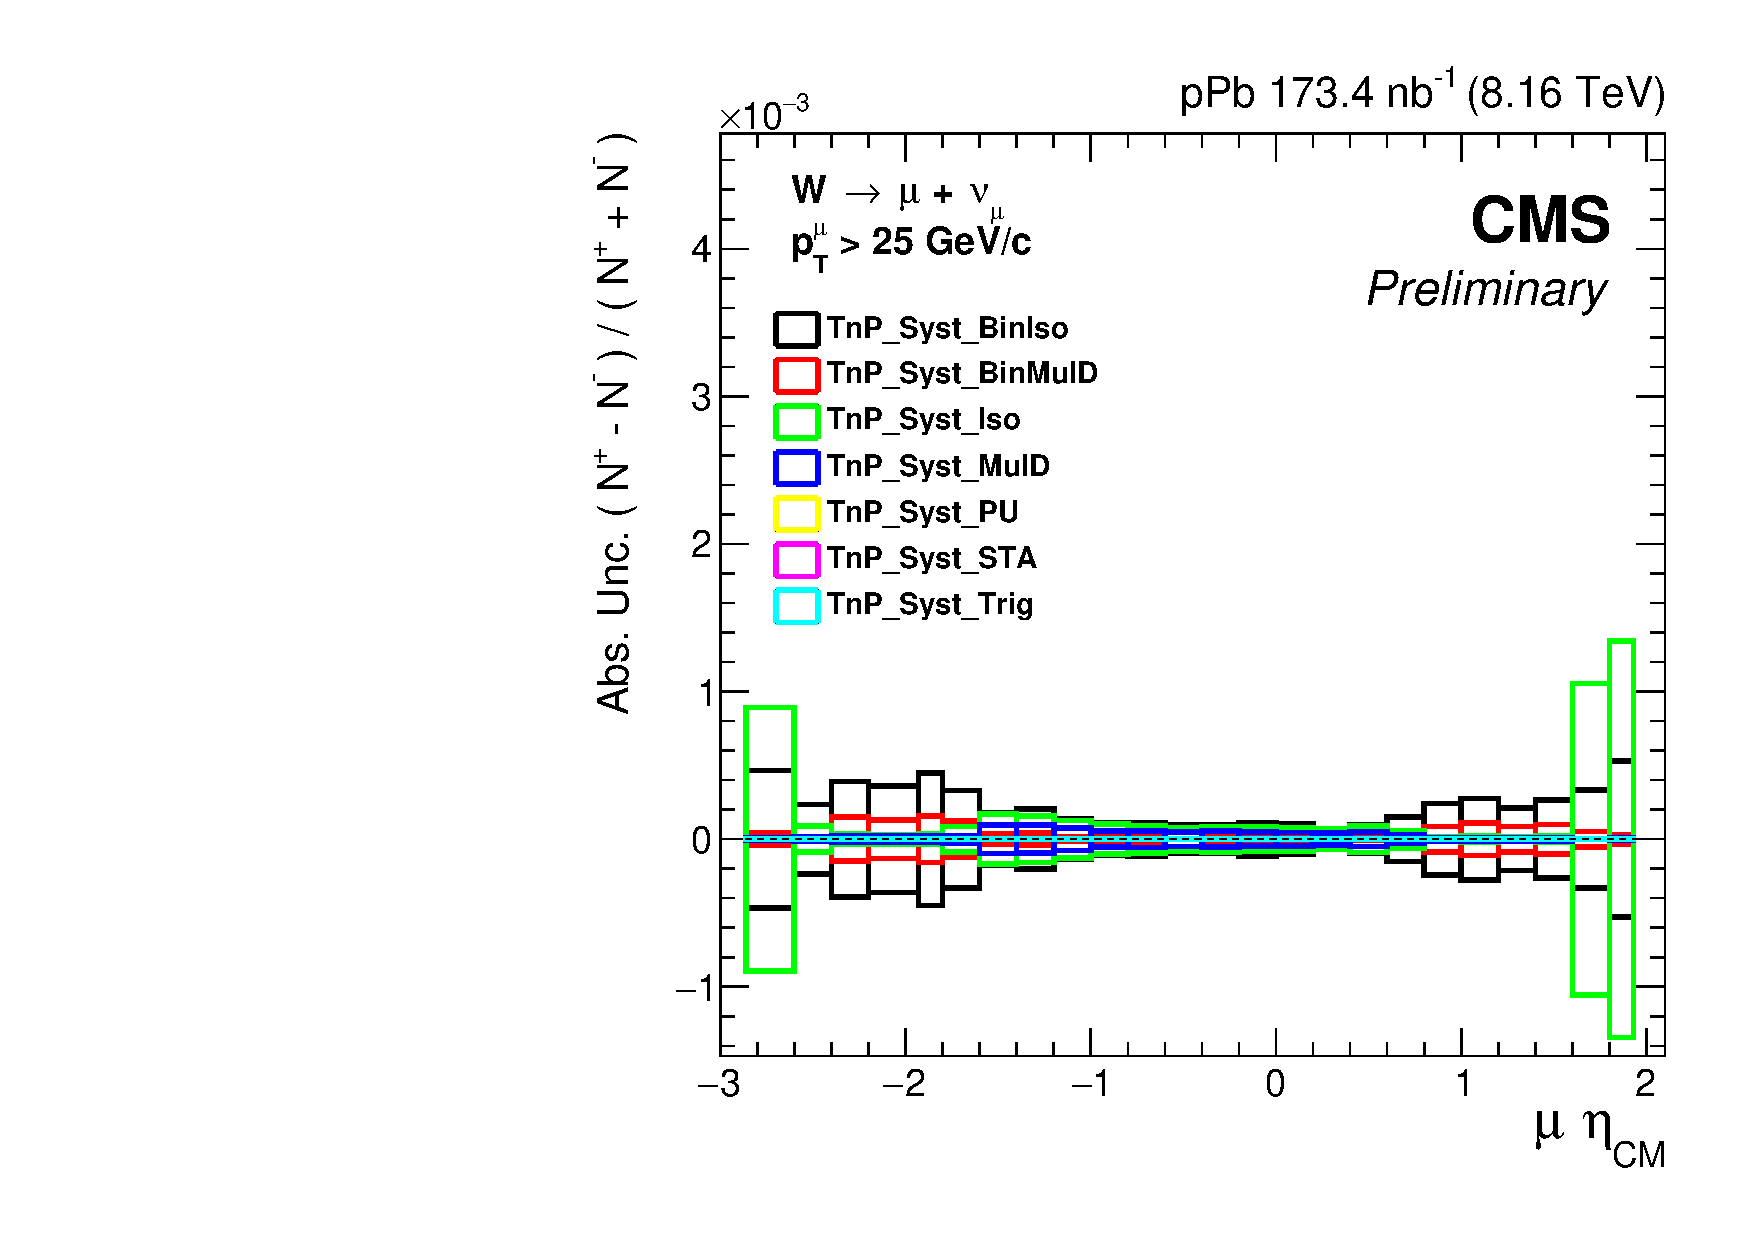
\includegraphics[width=0.29\textwidth]{Figures/WBoson/Analysis/Systematics/Combined/PA/Charge_Asymmetry/gr_WToMuInc_PA_Charge_Asymmetry_EffTnP_TnP_Syst.pdf}
 \end{center}
 \caption{Systematic variation corresponding to the TnP systematic components. The plots are divided as: \WToMuNuMi (top-left) and \WToMuNuPl (bottom-left) cross sections, $\W^{-}$ (top-middle) and $\W^{+}$ (bottom-middle) $R_{FB}$, and finally the \W $R_{FB}$ (top-right) and \W charge asymmetry (bottom-right).}
 \label{fig:Systematic_Eff_TnP_Syst}
\end{figure}


\begin{figure}[!htbp]
 \begin{center}
  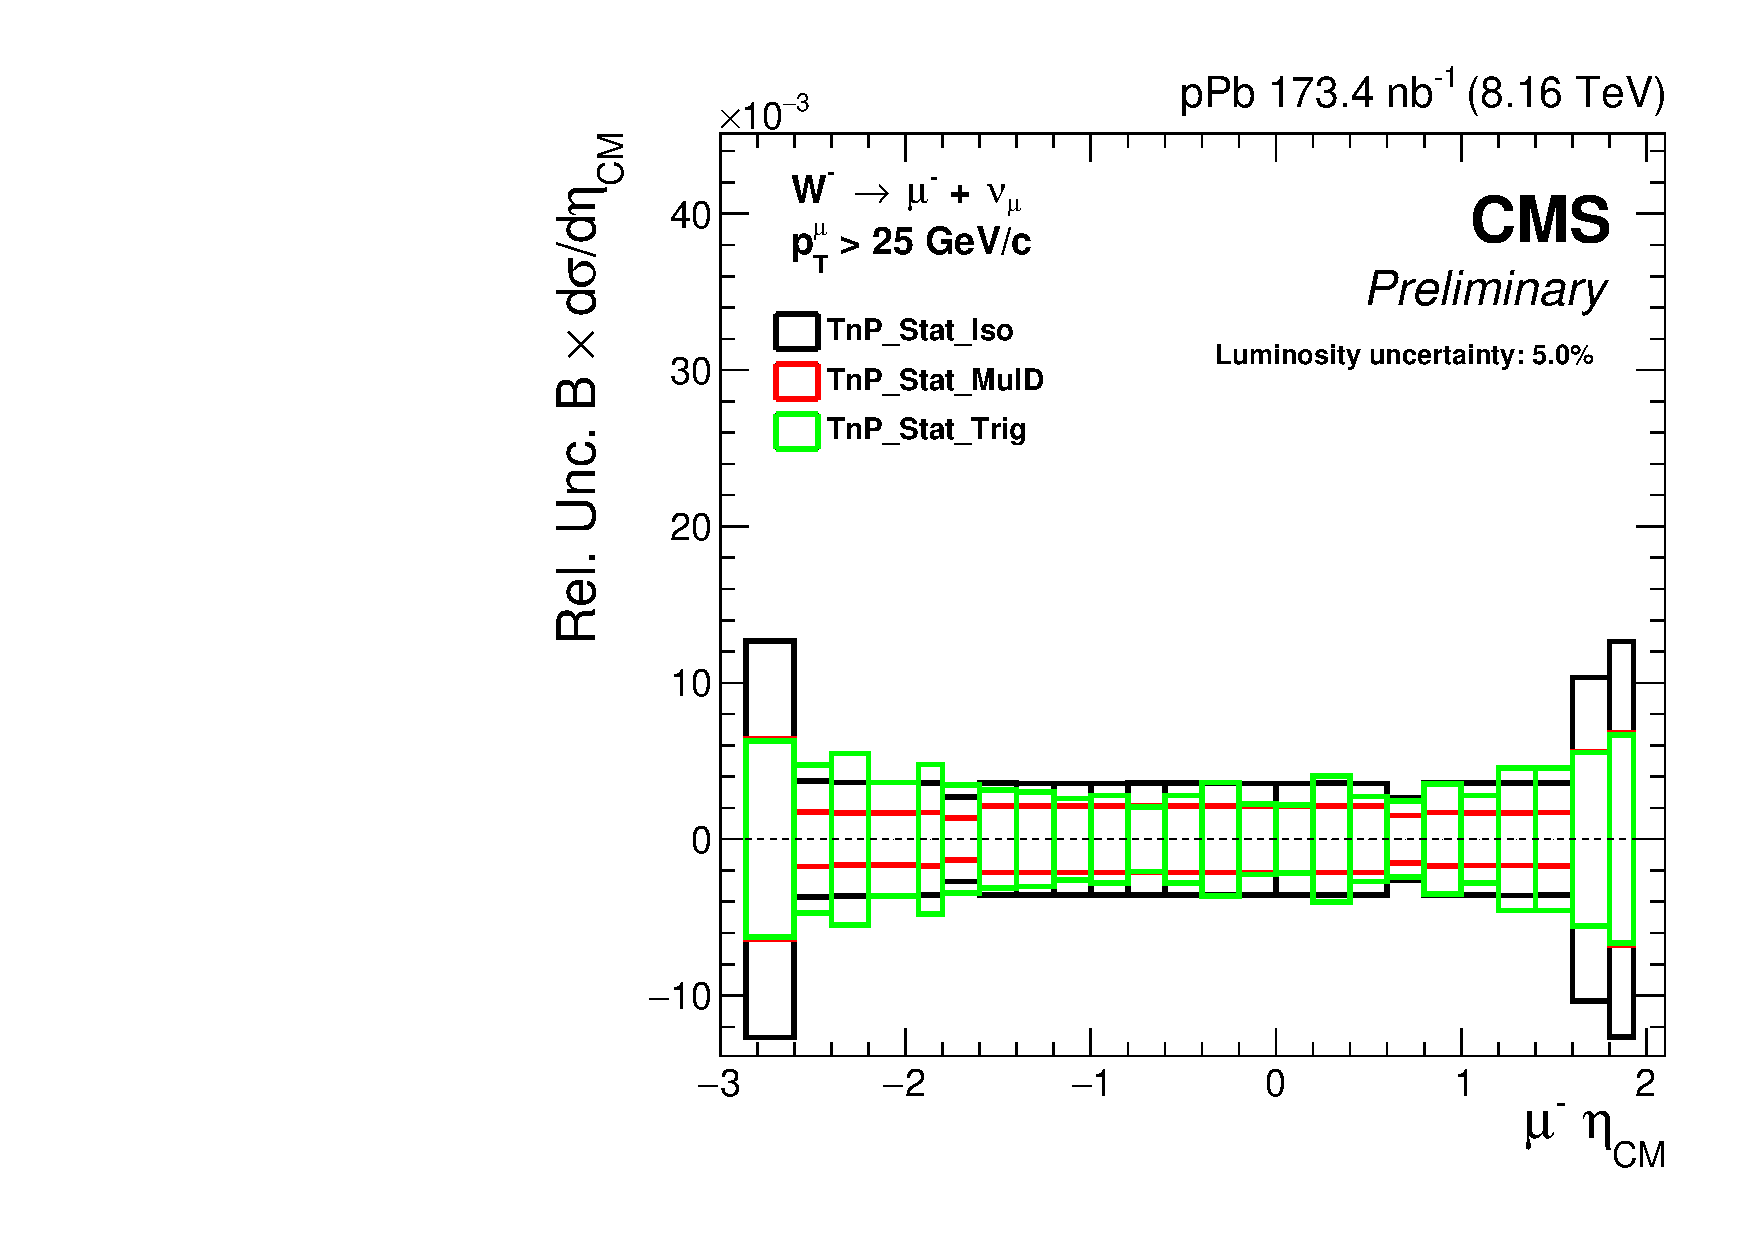
\includegraphics[width=0.29\textwidth]{Figures/WBoson/Analysis/Systematics/Combined/PA/Cross_Section/gr_WToMuMi_PA_Cross_Section_EffTnP_TnP_Stat.pdf}
  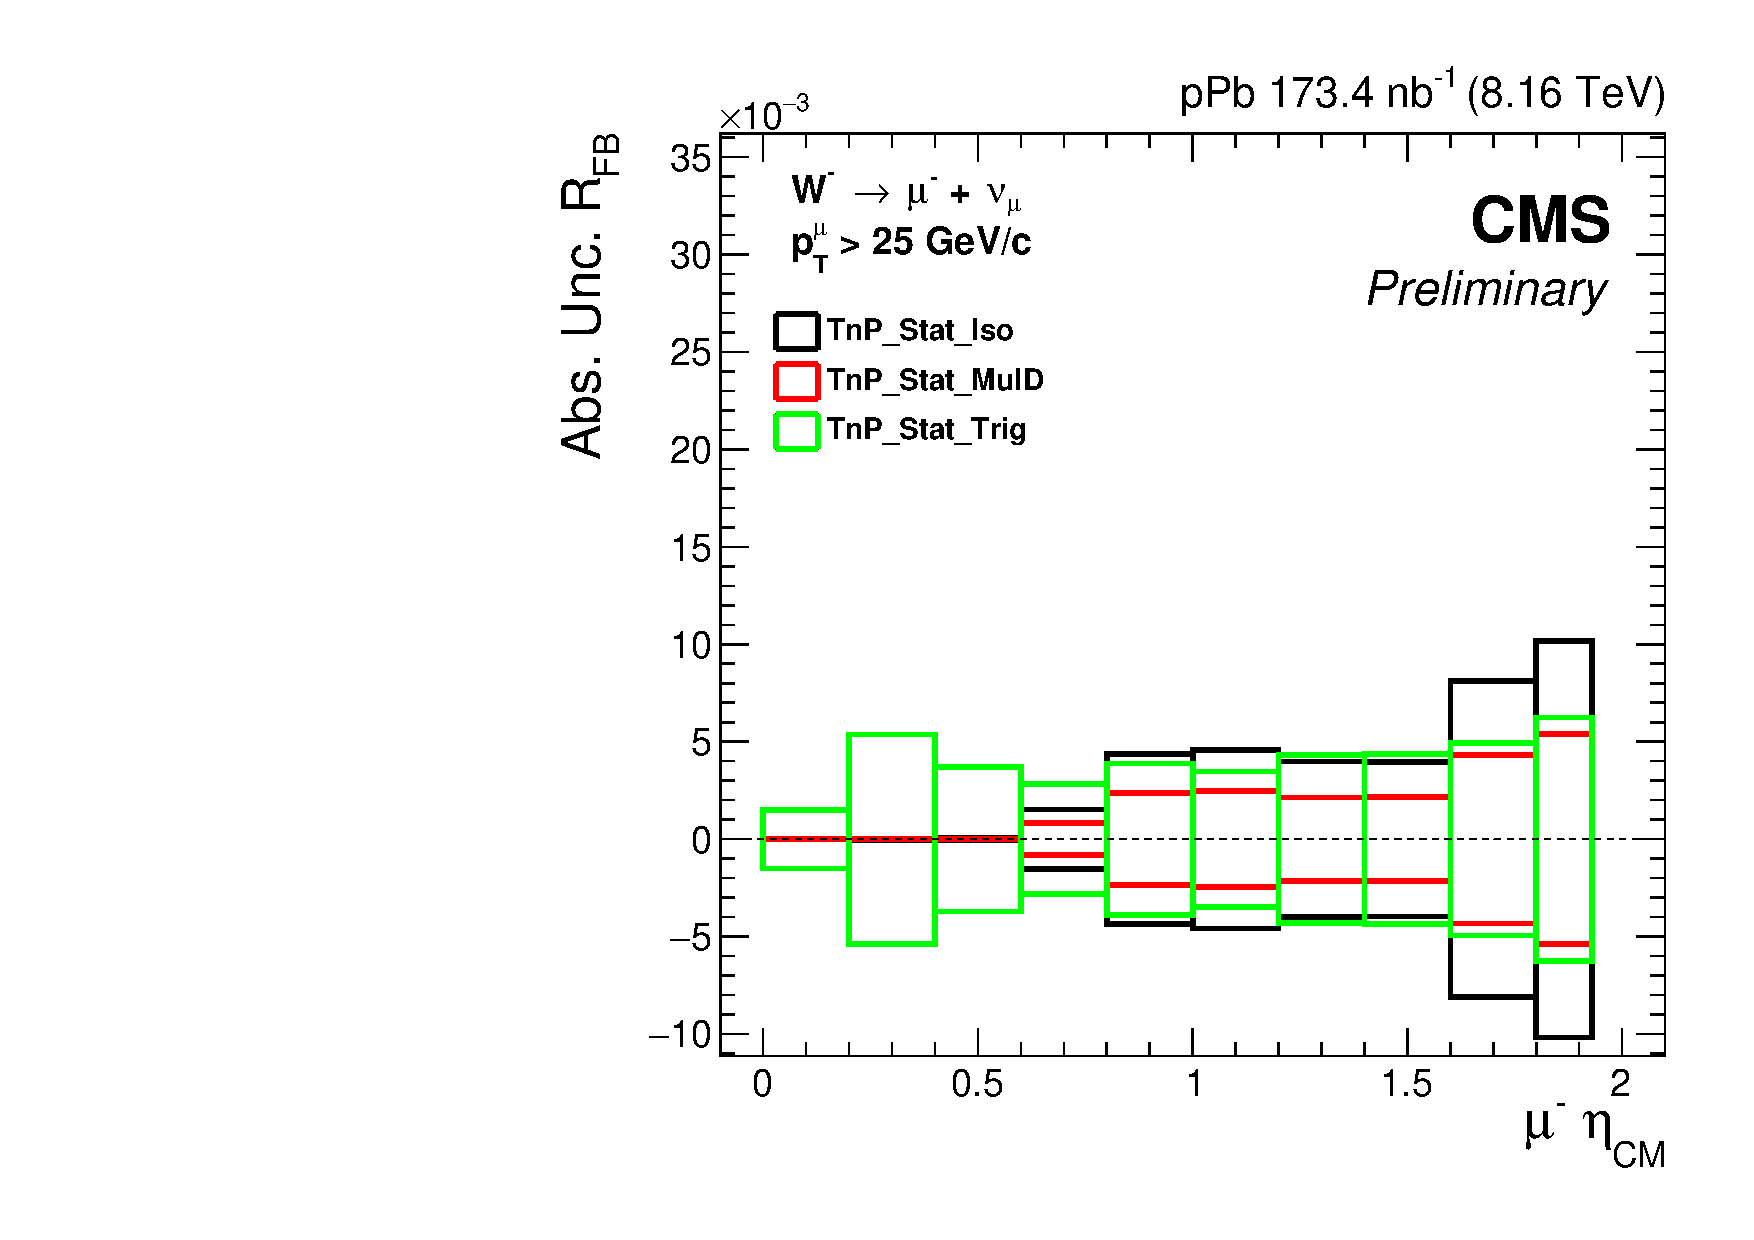
\includegraphics[width=0.29\textwidth]{Figures/WBoson/Analysis/Systematics/Combined/PA/ForwardBackward_Ratio/gr_WToMuMi_PA_ForwardBackward_Ratio_EffTnP_TnP_Stat.pdf}
  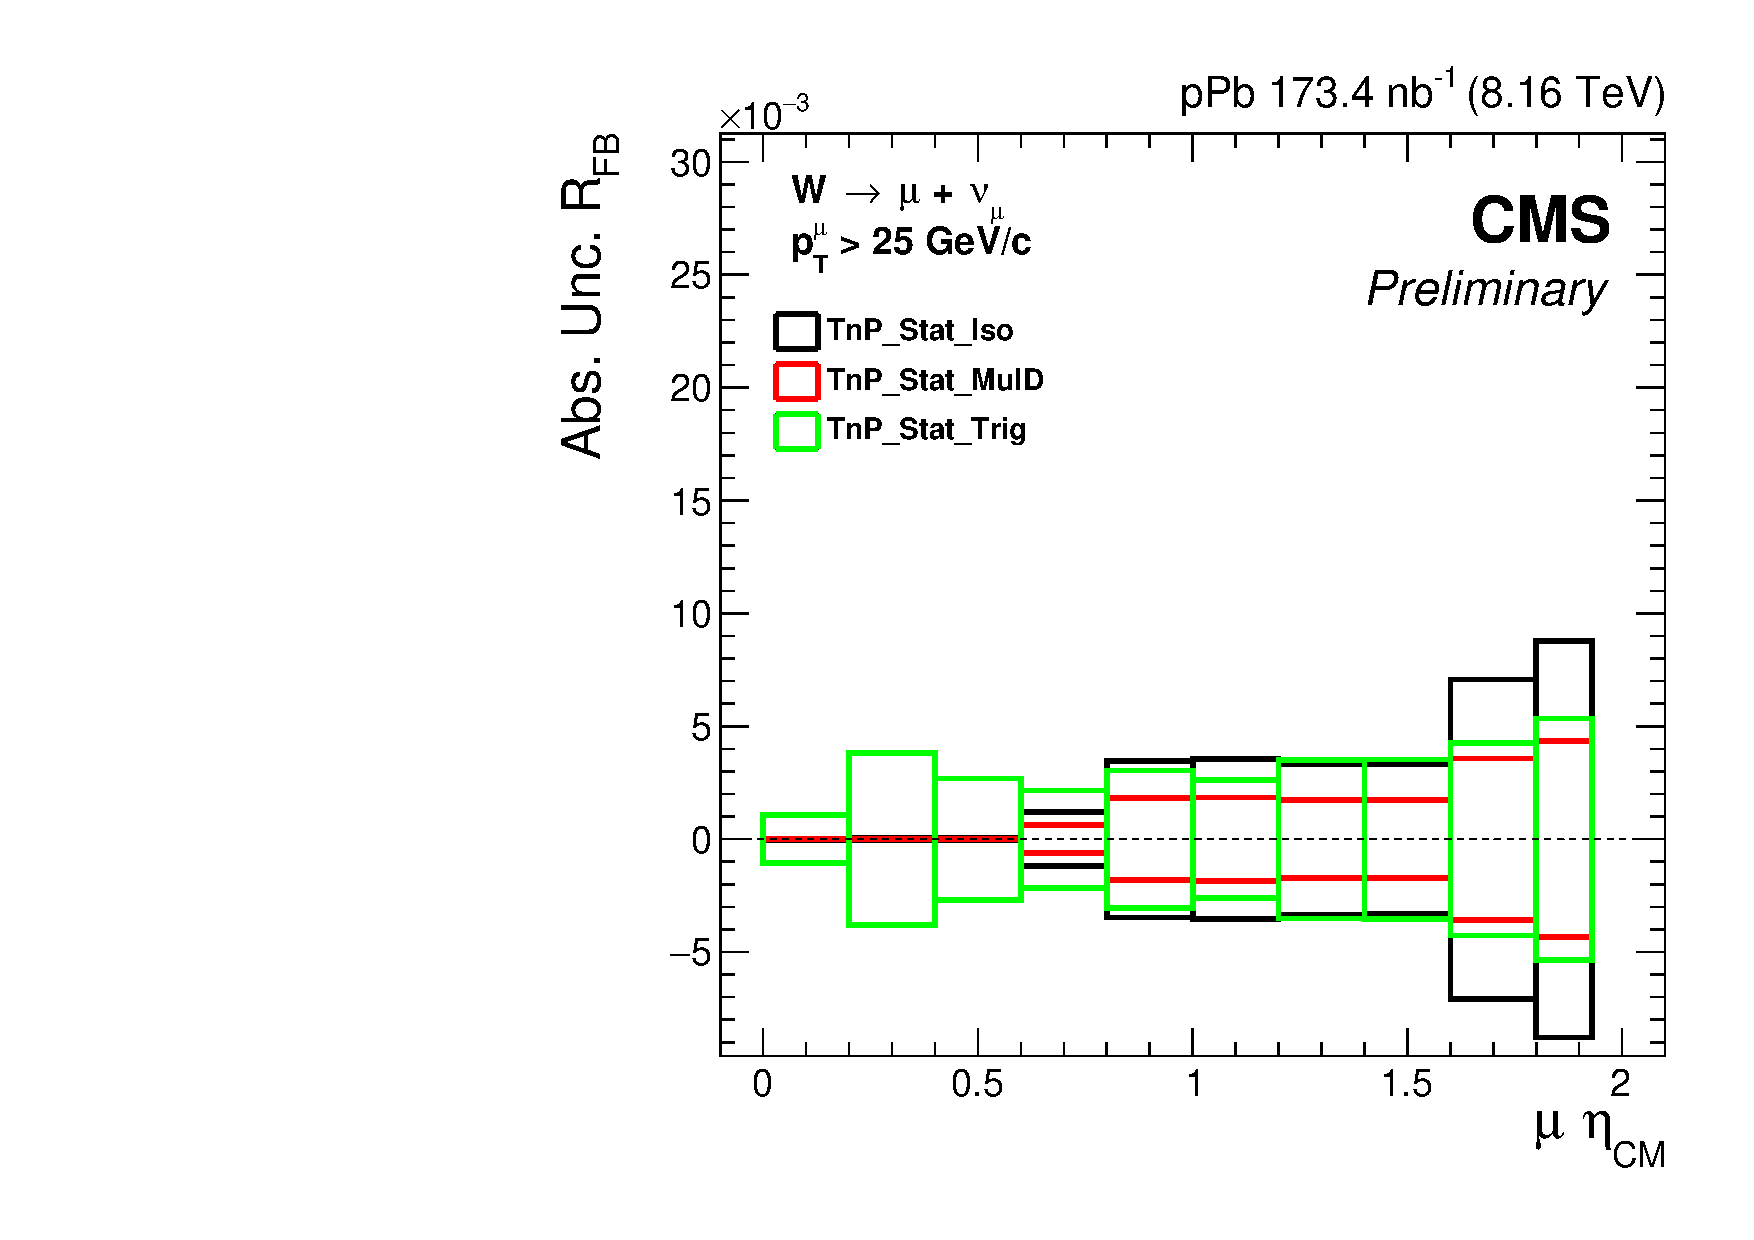
\includegraphics[width=0.29\textwidth]{Figures/WBoson/Analysis/Systematics/Combined/PA/ForwardBackward_Ratio/gr_WToMuInc_PA_ForwardBackward_Ratio_EffTnP_TnP_Stat.pdf}
%%
  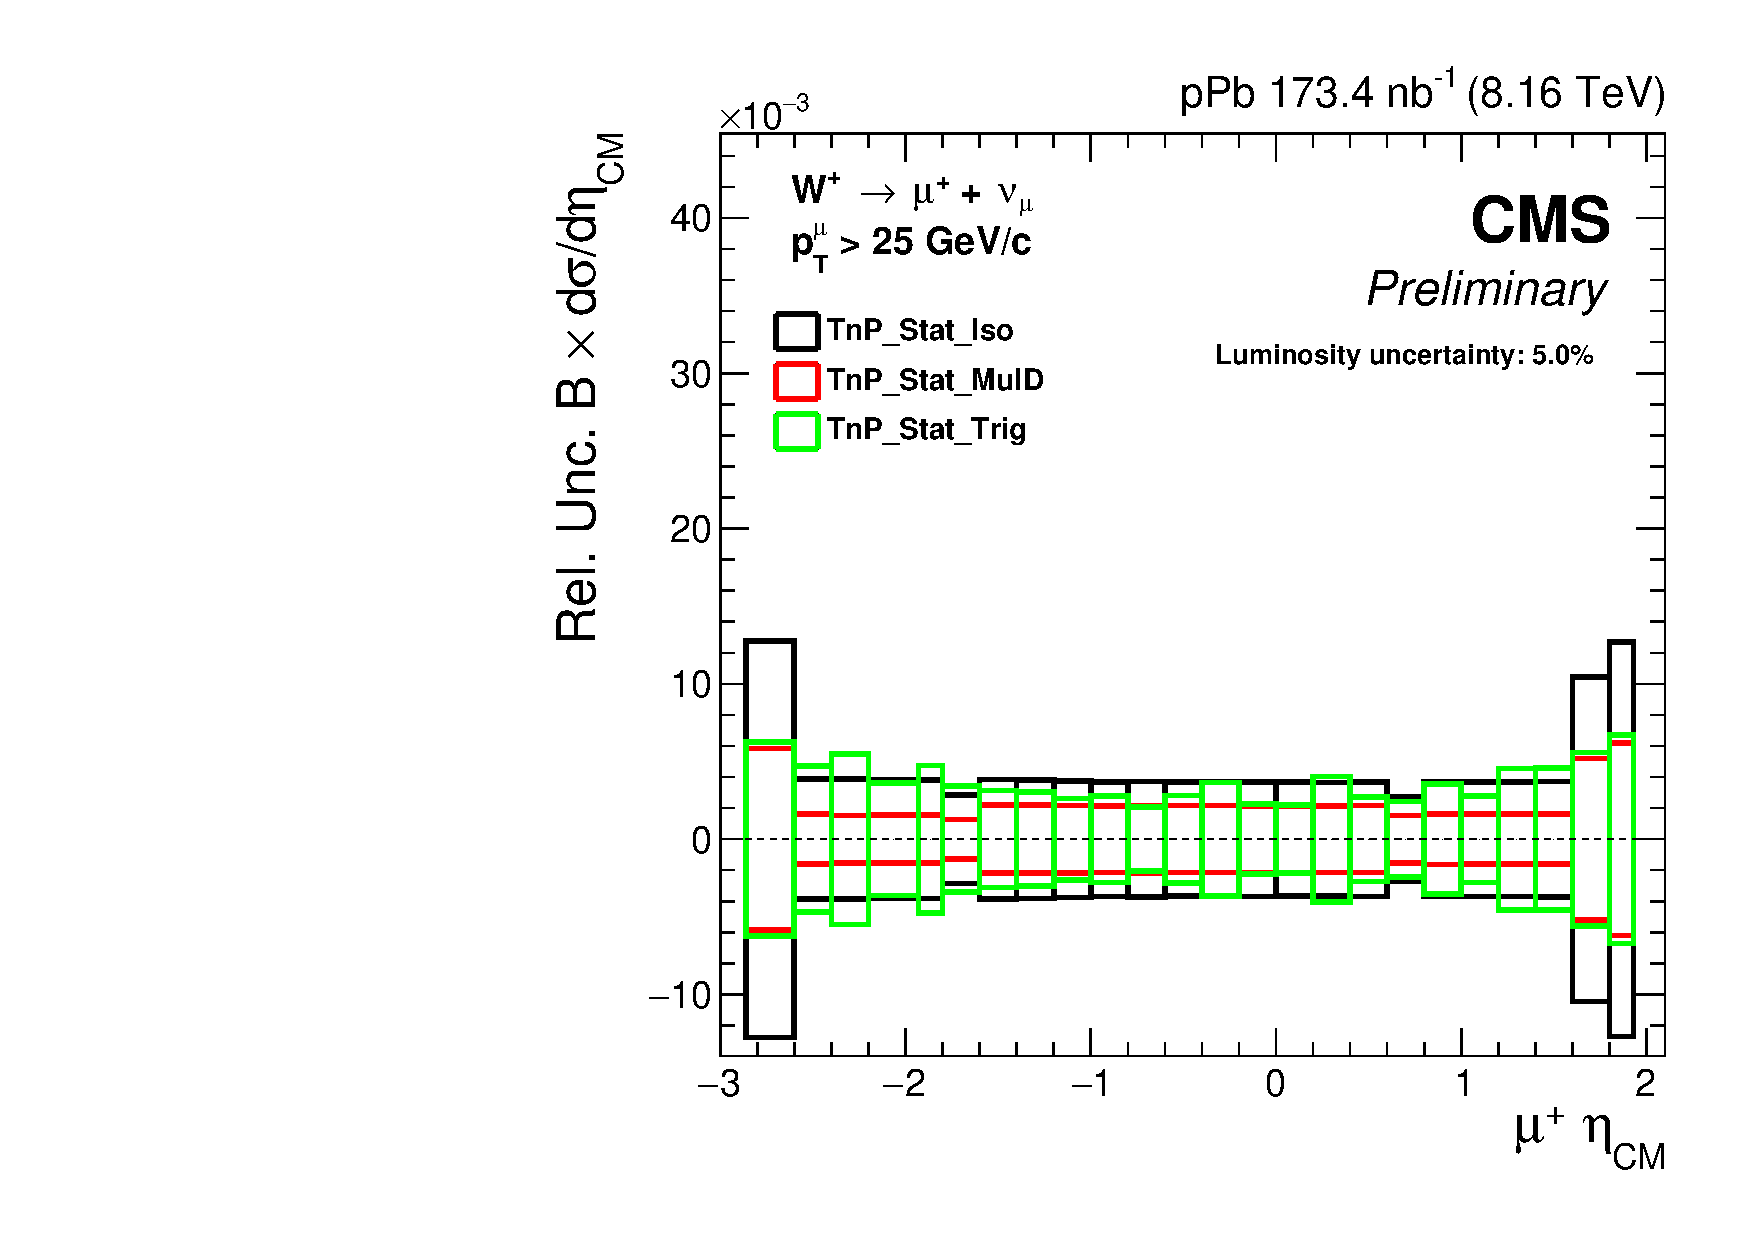
\includegraphics[width=0.29\textwidth]{Figures/WBoson/Analysis/Systematics/Combined/PA/Cross_Section/gr_WToMuPl_PA_Cross_Section_EffTnP_TnP_Stat.pdf}
  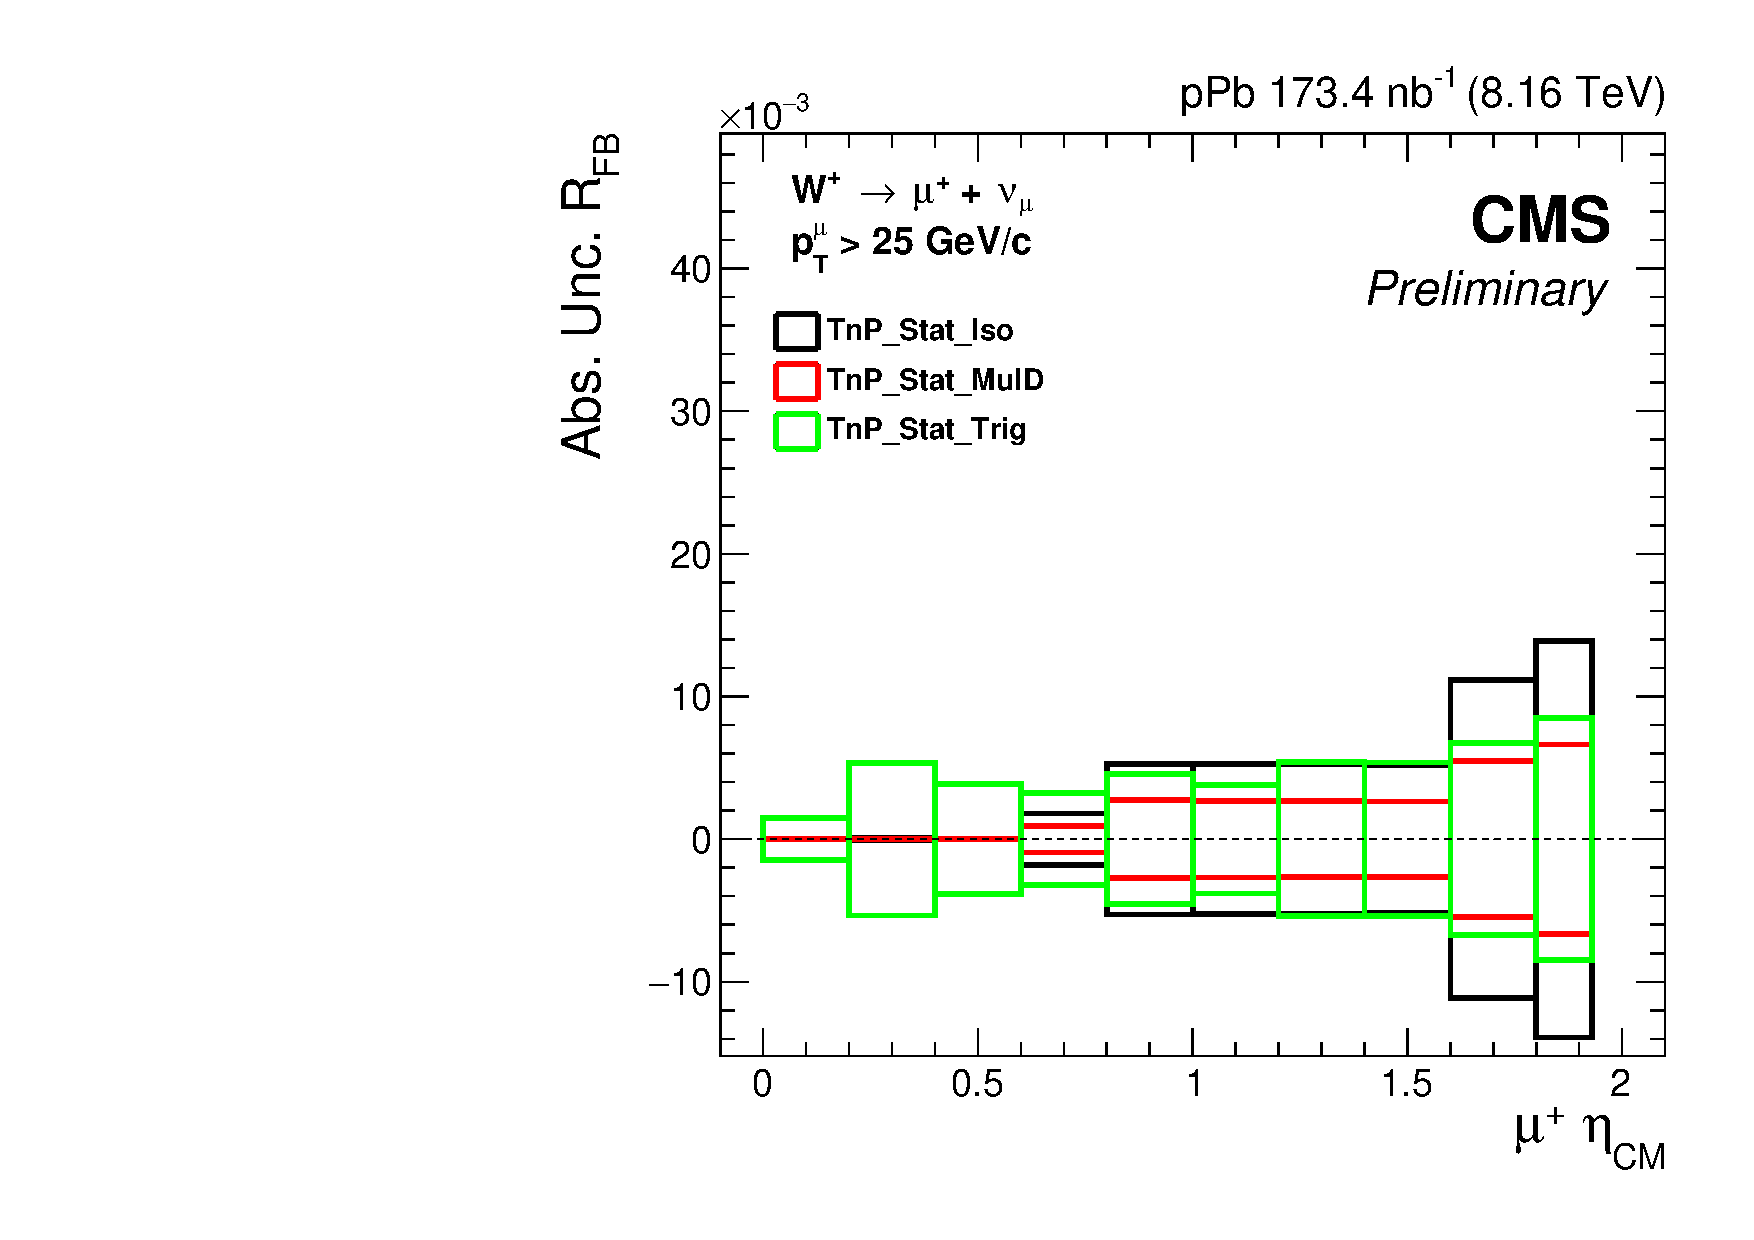
\includegraphics[width=0.29\textwidth]{Figures/WBoson/Analysis/Systematics/Combined/PA/ForwardBackward_Ratio/gr_WToMuPl_PA_ForwardBackward_Ratio_EffTnP_TnP_Stat.pdf}
  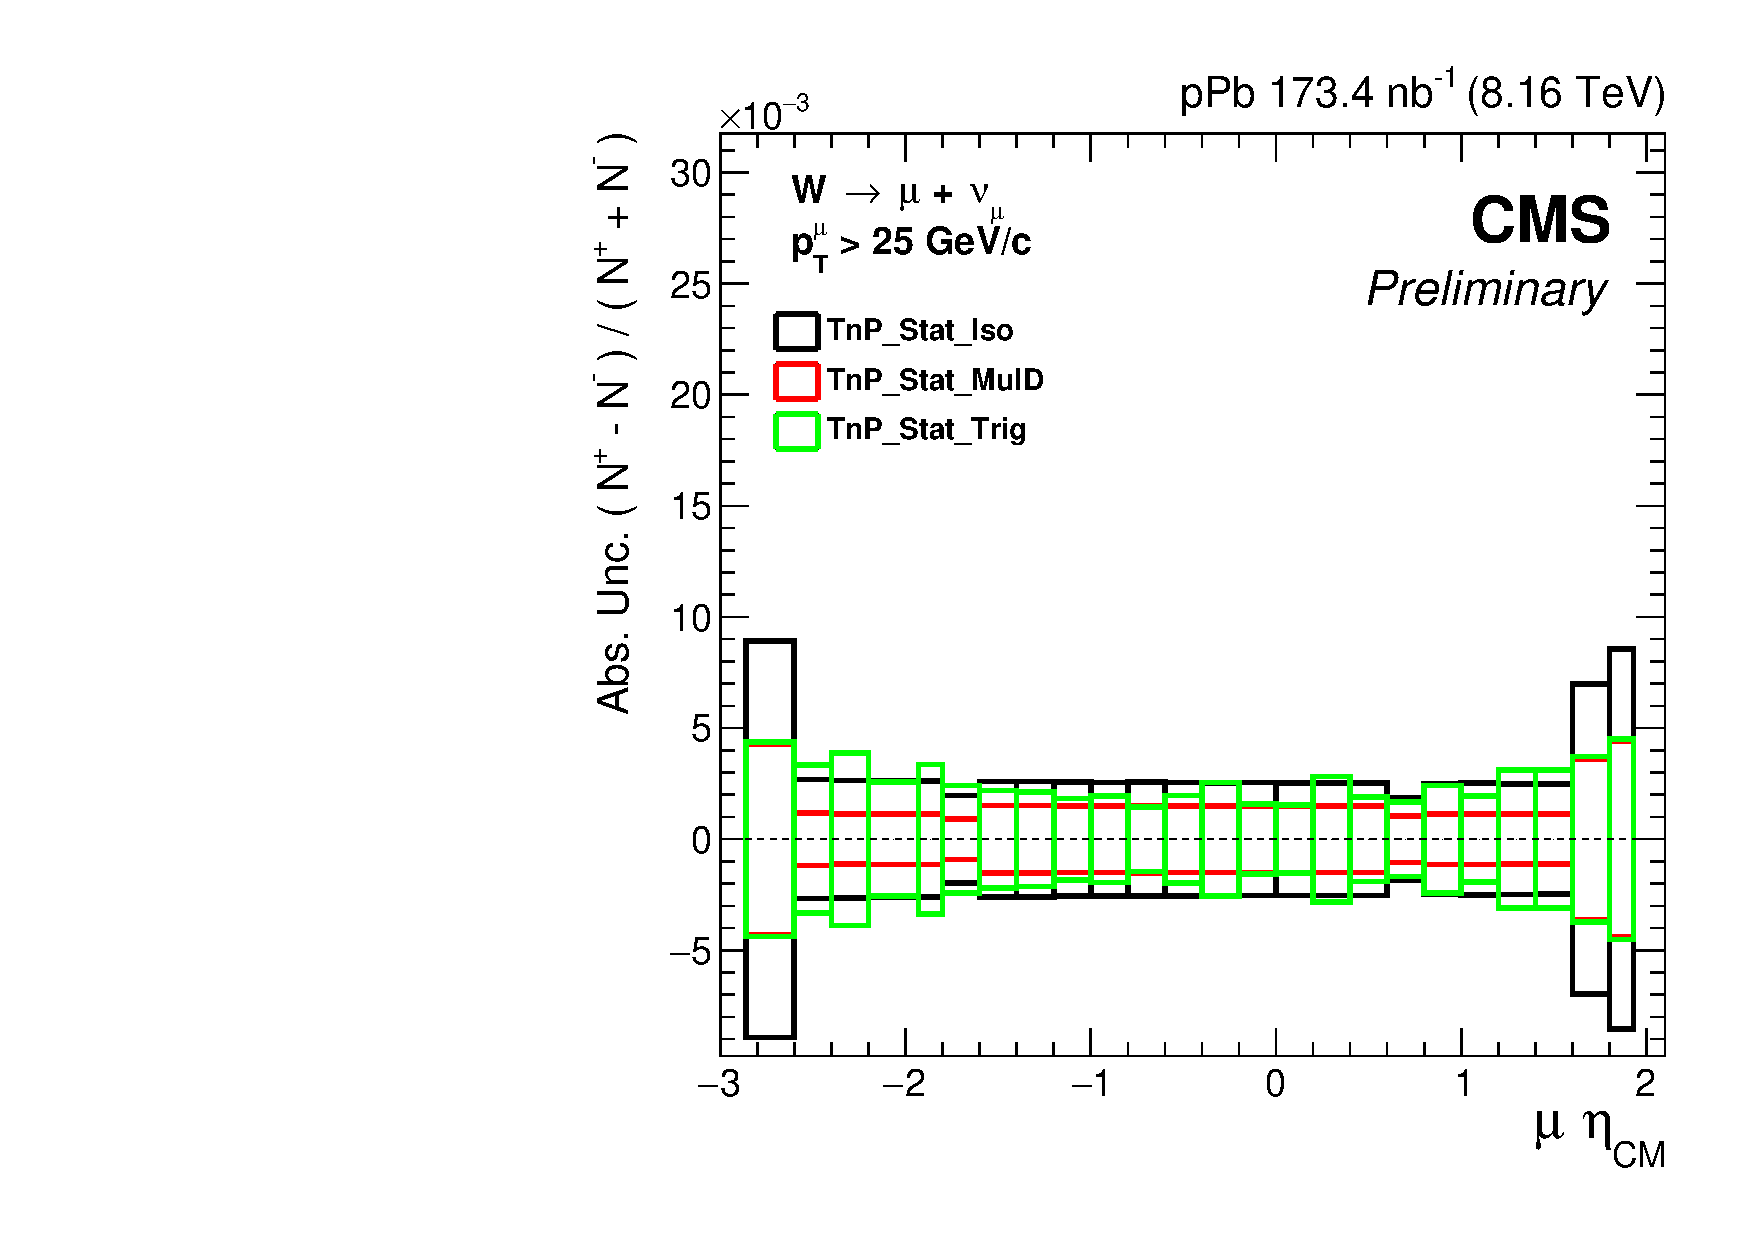
\includegraphics[width=0.29\textwidth]{Figures/WBoson/Analysis/Systematics/Combined/PA/Charge_Asymmetry/gr_WToMuInc_PA_Charge_Asymmetry_EffTnP_TnP_Stat.pdf}
 \end{center}
 \caption{Systematic variation corresponding to the TnP statistical components. The plots are divided as: \WToMuNuMi (top-left) and \WToMuNuPl (bottom-left) cross sections, $\W^{-}$ (top-middle) and $\W^{+}$ (bottom-middle) $R_{FB}$, and finally the \W $R_{FB}$ (top-right) and \W charge asymmetry (bottom-right).}
 \label{fig:Systematic_Eff_TnP_Stat}
\end{figure}


\clearpage
%%------------------------------------------------------------%%
\subsubsection{Choice of binning}


Since the \W signal distribution is parametrised using a binned MC template with a bin width of 2~\GeVc, the uncertainty on the signal template is determined by decreasing the bin width to 1~\GeVc. The systematic uncertainty is assigned for each $\eta_{CM}$ bin by taking the maximum difference between the nominal and the varied observables. The impact on the measurement of the cross sections, forward-backward ratios and charge asymmetry is shown in \fig{fig:Systematic_BinWidth}. The correlations bin-to-bin and between the positively and negatively charged muons is taken to be 100~$\%$.

\begin{figure}[htbp]
 \begin{center}
  \includegraphics[width=0.30\textwidth]{Figures/WBoson/Analysis/Systematics/Variation/PA/Cross_Section/gr_WToMuMi_PA_Cross_Section_EffTnP_BinWidth.pdf}
  \includegraphics[width=0.30\textwidth]{Figures/WBoson/Analysis/Systematics/Variation/PA/ForwardBackward_Ratio/gr_WToMuMi_PA_ForwardBackward_Ratio_EffTnP_BinWidth.pdf}
  \includegraphics[width=0.30\textwidth]{Figures/WBoson/Analysis/Systematics/Variation/PA/ForwardBackward_Ratio/gr_WToMuInc_PA_ForwardBackward_Ratio_EffTnP_BinWidth.pdf}
%%
  \includegraphics[width=0.30\textwidth]{Figures/WBoson/Analysis/Systematics/Variation/PA/Cross_Section/gr_WToMuPl_PA_Cross_Section_EffTnP_BinWidth.pdf}
  \includegraphics[width=0.30\textwidth]{Figures/WBoson/Analysis/Systematics/Variation/PA/ForwardBackward_Ratio/gr_WToMuPl_PA_ForwardBackward_Ratio_EffTnP_BinWidth.pdf}
  \includegraphics[width=0.30\textwidth]{Figures/WBoson/Analysis/Systematics/Variation/PA/Charge_Asymmetry/gr_WToMuInc_PA_Charge_Asymmetry_EffTnP_BinWidth.pdf}
 \end{center}
 \caption{Systematic variation corresponding to the choice of binning. The plots are divided as: \WToMuNuMi (top-left) and \WToMuNuPl (bottom-left) cross sections, $\W^{-}$ (top-middle) and $\W^{+}$ (bottom-middle) $R_{FB}$, and finally the \W $R_{FB}$ (top-right) and \W charge asymmetry (bottom-right). The values between square parenthesis represents the maximum and minimum relative uncertainty for the case of the cross sections and the absolute uncertainty for the $R_{FB}$ and charge asymmetry. The red lines shows the variations of the observables.}
 \label{fig:Systematic_BinWidth}
\end{figure}


\clearpage
%%------------------------------------------------------------%%
\subsubsection{QCD Background}

The systematic uncertainty in the QCD background originates from the uncertainty in the modeling of the multi-jet MET distribution in the signal region. The nominal procedure consist on fixing the parameters of the modified Rayleigh distribution from the fits extrapolated from data as explained in Sec.~\ref{sec:WBoson_Analysis_QCDBackground}. In order to estimate the uncertainty of the mismodeling of the QCD shape, both the parameters and the functional form are varied as explained in the following subsections.

\subsubsection{QCD Model Parameters}

The first source of systematic uncertainty reflects the possible mis-modelling of the QCD shape due to the $\eta_{CM}$ dependence of the QCD parameters. In order to check this, the parameters of the nominal QCD model are set free but constrained to the weighted RMS and mean value of the extrapolated results extracted in each $\eta_{CM}$ bin. The values used to constrain the $\sigma_{0}$,  $\sigma_{1}$ and  $\sigma_{2}$ parameters are shown in \tab{tab:QCDContrainPar}. The average over $\eta_{CM}$ bins of the difference between the final observables derived from the constrained fits and the nominal results is taken as the systematic error. This source of uncertainty is taken to be fully uncorrelated.

\begin{table}[!htbp]
  \begin{center}
  \begin{tabular}{|c|c|c|}\hline
  Parameter & $QCD \to \mu^{-}$ & $QCD \to \mu^{+}$ \\\hline
  $\sigma_{0}$ & 14.49$\pm$0.95 & 14.78$\pm$0.52 \\\hline
  $\sigma_{1}$ & 6.20$\pm$0.89 & 6.77$\pm$0.91\\\hline
  $\sigma_{2}$ & 0.50$\pm$0.73 & 0.48$\pm$0.57\\\hline
  \end{tabular}
  \end{center}
  \caption{QCD shape parameters, extracted from the weighted mean and RMS in muon $\eta_{CM}$ of the extrapolated values to the signal region.}
  \label{tab:QCDContrainPar}
\end{table}

Another systematic variation consists of changing the muon isolation point used to extrapolate the QCD parameters. In the nominal case, the isolation point of 0.03 was determined from the average muon isolation value in data inside the signal region. As an alternative case, the isolation distribution is checked in a QCD MC sample passing all the analysis cuts and the average isolation value is  determined to be approximately 0.08. Thus, the QCD parameters are recomputed by extrapolating them to an isolation point of 0.08, and the fits are redone by fixing the QCD parameters to the extrapolated values in the $\eta$ inclusive bin as in the nominal case. The new QCD parameters are listed in \tab{tab:QCDFixedPar_Iso0p08}. Since each bin varies independently, the uncertainty is taken to be fully uncorrelated.

\begin{table}[!htbp]
  \begin{center}
  \begin{tabular}{|c|c|c|}\hline
  Parameter & $QCD \to \mu^{-}$ & $QCD \to \mu^{+}$ \\\hline
  $\sigma_{0}$ & 14.67 & 14.79 \\\hline
  $\sigma_{1}$ & 6.28 & 6.71 \\\hline
  $\sigma_{2}$ & 0.50 & 0.49 \\\hline
  \end{tabular}
  \end{center}
  \caption{QCD shape parameters, extrapolated to the average isolation in a QCD MC sample passing all analysis cuts ($\text{iso} = 0.08$).}
  \label{tab:QCDFixedPar_Iso0p08}
\end{table}

The results of the systematic variations due to the QCD constrained fits and the re-extrapolated QCD parameters are shown in \fig{fig:Systematic_QCD_ConstrainMean} and \fig{fig:Systematic_QCD_Iso0p08}, respectively.

\begin{figure}[htbp]
 \begin{center}
  \includegraphics[width=0.26\textwidth]{Figures/WBoson/Analysis/Systematics/Variation/PA/Cross_Section/gr_WToMuMi_PA_Cross_Section_EffTnP_QCD_ConstrainMean_Avg.pdf}
  \includegraphics[width=0.26\textwidth]{Figures/WBoson/Analysis/Systematics/Variation/PA/ForwardBackward_Ratio/gr_WToMuMi_PA_ForwardBackward_Ratio_EffTnP_QCD_ConstrainMean_Avg.pdf}
  \includegraphics[width=0.26\textwidth]{Figures/WBoson/Analysis/Systematics/Variation/PA/ForwardBackward_Ratio/gr_WToMuInc_PA_ForwardBackward_Ratio_EffTnP_QCD_ConstrainMean_Avg.pdf}
%%
  \includegraphics[width=0.26\textwidth]{Figures/WBoson/Analysis/Systematics/Variation/PA/Cross_Section/gr_WToMuPl_PA_Cross_Section_EffTnP_QCD_ConstrainMean_Avg.pdf}
  \includegraphics[width=0.26\textwidth]{Figures/WBoson/Analysis/Systematics/Variation/PA/ForwardBackward_Ratio/gr_WToMuPl_PA_ForwardBackward_Ratio_EffTnP_QCD_ConstrainMean_Avg.pdf}
  \includegraphics[width=0.26\textwidth]{Figures/WBoson/Analysis/Systematics/Variation/PA/Charge_Asymmetry/gr_WToMuInc_PA_Charge_Asymmetry_EffTnP_QCD_ConstrainMean_Avg.pdf}
 \end{center}
 \caption{Systematic variation corresponding to the constrain fits. The plots are divided as: \WToMuNuMi (top-left) and \WToMuNuPl (bottom-left) cross sections, $\W^{-}$ (top-middle) and $\W^{+}$ (bottom-middle) $R_{FB}$, and finally the \W $R_{FB}$ (top-right) and \W charge asymmetry (bottom-right). The values between square parenthesis represents the maximum and minimum relative uncertainty for the case of the cross sections and the absolute uncertainty for the $R_{FB}$ and charge asymmetry. The red lines represent the variations of the observables in each bin.}
 \label{fig:Systematic_QCD_ConstrainMean}
\end{figure}

\begin{figure}[htbp]
 \begin{center}
  \includegraphics[width=0.26\textwidth]{Figures/WBoson/Analysis/Systematics/Variation/PA/Cross_Section/gr_WToMuMi_PA_Cross_Section_EffTnP_QCD_Iso0p08.pdf}
  \includegraphics[width=0.26\textwidth]{Figures/WBoson/Analysis/Systematics/Variation/PA/ForwardBackward_Ratio/gr_WToMuMi_PA_ForwardBackward_Ratio_EffTnP_QCD_Iso0p08.pdf}
  \includegraphics[width=0.26\textwidth]{Figures/WBoson/Analysis/Systematics/Variation/PA/ForwardBackward_Ratio/gr_WToMuInc_PA_ForwardBackward_Ratio_EffTnP_QCD_Iso0p08.pdf}
%%
  \includegraphics[width=0.26\textwidth]{Figures/WBoson/Analysis/Systematics/Variation/PA/Cross_Section/gr_WToMuPl_PA_Cross_Section_EffTnP_QCD_Iso0p08.pdf}
  \includegraphics[width=0.26\textwidth]{Figures/WBoson/Analysis/Systematics/Variation/PA/ForwardBackward_Ratio/gr_WToMuPl_PA_ForwardBackward_Ratio_EffTnP_QCD_Iso0p08.pdf}
  \includegraphics[width=0.26\textwidth]{Figures/WBoson/Analysis/Systematics/Variation/PA/Charge_Asymmetry/gr_WToMuInc_PA_Charge_Asymmetry_EffTnP_QCD_Iso0p08.pdf}
 \end{center}
 \caption{Systematic variation corresponding to the constrained fits. The plots are divided as: \WToMuNuMi (top-left) and \WToMuNuPl (bottom-left) cross sections, $\W^{-}$ (top-middle) and $\W^{+}$ (bottom-middle) $R_{FB}$, and finally the \W $R_{FB}$ (top-right) and \W charge asymmetry (bottom-right). The values between square parenthesis represents the maximum and minimum relative uncertainty for the case of the cross sections and the absolute uncertainty for the $R_{FB}$ and charge asymmetry. The red lines represent the variations of the observables in each bin.}
 \label{fig:Systematic_QCD_Iso0p08}
\end{figure}

\clearpage
\subsubsection{QCD Functional Form}

To assign a systematic uncertainty due to the assumed functional form for modelling the QCD MET distribution, the shape of the QCD is described using a different model. The alternative MET distribution function used, taken from \cite{HIN-13-007}, is shown in \eq{eq:QCDMultiJet}. 

\begin{equation}\label{eq:QCDMultiJet}
f(x) = (x+x_0)^\alpha \exp(\beta\sqrt{x+x_0})
\end{equation}

The extrapolation procedure explained in \sect{sec:WBoson_Analysis_QCDBackground} is redone using the alternative model, and the results are summarized in the Appendix~\ref{app:QCD_Alternative}. All the fits are remade using the new QCD functional form fixed to the QCD parameters extrapolated in the inclusive $\eta_{CM}$ bin. The difference between the final observables derived using the alternative QCD PDF and the nominal results is taken as the systematic error due to mis-modeling of the QCD shape. The bin-to-bin correlation for this uncertainty is taken to be fully uncorrelated.

The variations on the final observables due to the use of the alternative QCD PDF are shown in \fig{fig:Systematic_QCD_MultiJet}.

\begin{figure}[htbp]
 \begin{center}
  \includegraphics[width=0.30\textwidth]{Figures/WBoson/Analysis/Systematics/Variation/PA/Cross_Section/gr_WToMuMi_PA_Cross_Section_EffTnP_QCD_MultiJet.pdf}
  \includegraphics[width=0.30\textwidth]{Figures/WBoson/Analysis/Systematics/Variation/PA/ForwardBackward_Ratio/gr_WToMuMi_PA_ForwardBackward_Ratio_EffTnP_QCD_MultiJet.pdf}
  \includegraphics[width=0.30\textwidth]{Figures/WBoson/Analysis/Systematics/Variation/PA/ForwardBackward_Ratio/gr_WToMuInc_PA_ForwardBackward_Ratio_EffTnP_QCD_MultiJet.pdf}
%%
  \includegraphics[width=0.30\textwidth]{Figures/WBoson/Analysis/Systematics/Variation/PA/Cross_Section/gr_WToMuPl_PA_Cross_Section_EffTnP_QCD_MultiJet.pdf}
  \includegraphics[width=0.30\textwidth]{Figures/WBoson/Analysis/Systematics/Variation/PA/ForwardBackward_Ratio/gr_WToMuPl_PA_ForwardBackward_Ratio_EffTnP_QCD_MultiJet.pdf}
  \includegraphics[width=0.30\textwidth]{Figures/WBoson/Analysis/Systematics/Variation/PA/Charge_Asymmetry/gr_WToMuInc_PA_Charge_Asymmetry_EffTnP_QCD_MultiJet.pdf}
 \end{center}
 \caption{Systematic variation corresponding to the alternative QCD background model. The plots are divided as: \WToMuNuMi (top-left) and \WToMuNuPl (bottom-left) cross sections, $\W^{-}$ (top-middle) and $\W^{+}$ (bottom-middle) $R_{FB}$, and finally the \W $R_{FB}$ (top-right) and \W charge asymmetry (bottom-right). The values between square parenthesis represents the maximum and minimum relative uncertainty for the case of the cross sections and the absolute uncertainty for the $R_{FB}$ and charge asymmetry. The red lines represent the variations of the observables in each bin.}
 \label{fig:Systematic_QCD_MultiJet}
\end{figure}

\clearpage
%%------------------------------------------------------------%%
\subsubsection{EWK Background}

The different sources of EWK background are described using templates derived from the MC \POWHEG samples. Since the simulations are scaled to the luminosity recorded by CMS by using the cross-section of each EWK process, a systematic uncertainty is assigned to each source by varying their cross sections as explained below.

\subsubsection{\texorpdfstring{\DYToMuMu}\ Background}\label{sec:WBoson_Analysis_Systematic_DYToMuMu}

When performing the fits, the ratio of the \DYToMuMu background over the signal yields is fixed to the corresponding value extracted from the simulation. The MC sample is normalized to match the integrated luminosity in data using the \DYToMuMu and \WToMuNu NLO cross sections derived from \POWHEG.

The uncertainty on the $\W/\Z$ ratio is estimated using MCFM~\cite{MCFM8} at NLO with CT14+EPPS16 \cite{CT14,EPPS16}. More precisely, the ratio is between the \WToMuNu cross section and the \DYToMuMu ($M\in [15,600]\GeVcc$) cross section, both with muon kinematic cuts ($\pt^{\mu} > 25$~\GeVc for \W and $\pt^{\mu} > 15$~\GeVc for \DY). This PDF uncertainty is propagated in the standard way for Hessian PDF sets (Eq. 20 of Ref.~\cite{PDF4LHC}). The results for the full CT14+EPPS16 uncertainty are the following:

\begin{eqnarray}
 \W^{+} / \Z = 3.455^{+0.038}_{-0.044} \\
 \W^{-} / \Z = 2.784^{+0.021}_{-0.020}
\end{eqnarray}

corresponding to a relative uncertainty of $0.8\%$ for $Z/\W^{-}$ and $1.3\%$ for $Z/\W^{+}$.

Since the cross sections in the muon channel depend on the branching ratio associated to each process, their uncertainty has to be also taken into account. The values of the branching ratios are extracted from the Particle Data Group (PDG) database \cite{PDG}, and correspond to $\textrm{BR}(\ZToMuMu) = (3.366 \pm 0.007)\%$ and $\textrm{BR}(\WToMuNu) = (10.63 \pm 0.15)\%$, which gives a relative uncertainty on the ratio of $\Z/\W$ branching ratios of $1.4\%$. Summing in quadrature the MCFM uncertainties with the ones derived from the branching ratios, one gets a total relative uncertainty for $\Z/\PWp$ of $1.6\%$ and for $\Z/\PWm$ of $1.9\%$. To be conservative the systematic variation is fixed to $2\%$ overall.

Therefore, the systematic uncertainty due to the \DYToMuMu background is determined by varying the \DYToMuMu cross section by $2\%$ up and down when performing the fits. The systematic uncertainty in each $\eta_{CM}$ bin is derived by taking the maximum difference between the nominal and the up/down variations. The bin-to-bin correlations in charge and pseudorapidity are taken to be 100\%.

The impact on each observable of varying the ratio of \DYToMuMu over \WToMuNu cross sections is shown in \fig{fig:Systematic_DYToMuMu}.

\begin{figure}[htbp]
 \begin{center}
  \includegraphics[width=0.30\textwidth]{Figures/WBoson/Analysis/Systematics/Variation/PA/Cross_Section/gr_WToMuMi_PA_Cross_Section_EffTnP_XSection_DYToMuMu.pdf}
  \includegraphics[width=0.30\textwidth]{Figures/WBoson/Analysis/Systematics/Variation/PA/ForwardBackward_Ratio/gr_WToMuMi_PA_ForwardBackward_Ratio_EffTnP_XSection_DYToMuMu.pdf}
  \includegraphics[width=0.30\textwidth]{Figures/WBoson/Analysis/Systematics/Variation/PA/ForwardBackward_Ratio/gr_WToMuInc_PA_ForwardBackward_Ratio_EffTnP_XSection_DYToMuMu.pdf}
%%
  \includegraphics[width=0.30\textwidth]{Figures/WBoson/Analysis/Systematics/Variation/PA/Cross_Section/gr_WToMuPl_PA_Cross_Section_EffTnP_XSection_DYToMuMu.pdf}
  \includegraphics[width=0.30\textwidth]{Figures/WBoson/Analysis/Systematics/Variation/PA/ForwardBackward_Ratio/gr_WToMuPl_PA_ForwardBackward_Ratio_EffTnP_XSection_DYToMuMu.pdf}
  \includegraphics[width=0.30\textwidth]{Figures/WBoson/Analysis/Systematics/Variation/PA/Charge_Asymmetry/gr_WToMuInc_PA_Charge_Asymmetry_EffTnP_XSection_DYToMuMu.pdf}
 \end{center}
 \caption{Systematic variation corresponding to the \DYToMuMu background contribution. The plots are divided as: \WToMuNuMi (top-left) and \WToMuNuPl (bottom-left) cross sections, $\W^{-}$ (top-middle) and $\W^{+}$ (bottom-middle) $R_{FB}$, and finally the \W $R_{FB}$ (top-right) and \W charge asymmetry (bottom-right). The values between square parenthesis represents the maximum and minimum relative uncertainty for the case of the cross sections and the absolute uncertainty for the $R_{FB}$ and charge asymmetry. The red and blue lines represent the up and down variations, respectively.}
 \label{fig:Systematic_DYToMuMu}
\end{figure}

\clearpage
\subsubsection{\texorpdfstring{\DYToTauTau}\ Background}

The ratio of the \DYToTauTau background over the signal raw yields is also fixed to the values derived from the corrected MC samples. Its uncertainty is considered to be the same as the 2$\%$ uncertainty determined for the \DYToMuMu background as detailed in \sect{sec:WBoson_Analysis_Systematic_DYToMuMu}.

To account for the difference in the \Z branching ratios to leptons, the current values are taken from the PDG \cite{PDG}. They correspond to $\textrm{BR}(\ZToTauTau) = (3.370 \pm 0.008)\%$ and $\textrm{BR}(\ZToMuMu) = (3.366 \pm 0.007)\%$, which represents a relative uncertainty on the ratio of $\ZToTauTau/\ZToMuMu$ branching ratios of $0.3\%$. Since the relative uncertainty of the \Z branching ratios is very small compared to the \DYToMuMu background uncertainty, it is not considered.

Hence, the \DYToTauTau cross section is varied by $2\%$ up and down when performing the fits. The systematic uncertainty in each $\eta_{CM}$ bin is derived by taking the maximum difference between the nominal and the up/down variations. The bin-to-bin correlations are taken to be 100\% both in charge and pseudorapidity.

The impact on each observable of varying the ratio of \DYToTauTau over \WToMuNu cross sections is shown in \fig{fig:Systematic_DYToTauTau}.

\begin{figure}[htbp]
 \begin{center}
  \includegraphics[width=0.30\textwidth]{Figures/WBoson/Analysis/Systematics/Variation/PA/Cross_Section/gr_WToMuMi_PA_Cross_Section_EffTnP_XSection_DYToTauTau.pdf}
  \includegraphics[width=0.30\textwidth]{Figures/WBoson/Analysis/Systematics/Variation/PA/ForwardBackward_Ratio/gr_WToMuMi_PA_ForwardBackward_Ratio_EffTnP_XSection_DYToTauTau.pdf}
  \includegraphics[width=0.30\textwidth]{Figures/WBoson/Analysis/Systematics/Variation/PA/ForwardBackward_Ratio/gr_WToMuInc_PA_ForwardBackward_Ratio_EffTnP_XSection_DYToTauTau.pdf}
%%
  \includegraphics[width=0.30\textwidth]{Figures/WBoson/Analysis/Systematics/Variation/PA/Cross_Section/gr_WToMuPl_PA_Cross_Section_EffTnP_XSection_DYToTauTau.pdf}
  \includegraphics[width=0.30\textwidth]{Figures/WBoson/Analysis/Systematics/Variation/PA/ForwardBackward_Ratio/gr_WToMuPl_PA_ForwardBackward_Ratio_EffTnP_XSection_DYToTauTau.pdf}
  \includegraphics[width=0.30\textwidth]{Figures/WBoson/Analysis/Systematics/Variation/PA/Charge_Asymmetry/gr_WToMuInc_PA_Charge_Asymmetry_EffTnP_XSection_DYToTauTau.pdf}
 \end{center}
 \caption{Systematic variation corresponding to the \DYToTauTau background contribution. The plots are divided as: \WToMuNuMi (top-left) and \WToMuNuPl (bottom-left) cross sections, $\W^{-}$ (top-middle) and $\W^{+}$ (bottom-middle) $R_{FB}$, and finally the \W $R_{FB}$ (top-right) and \W charge asymmetry (bottom-right). The values between square parenthesis represents the maximum and minimum relative uncertainty for the case of the cross sections and the absolute uncertainty for the $R_{FB}$ and charge asymmetry. The red and blue lines represent the up and down variations, respectively.}
 \label{fig:Systematic_DYToTauTau}
\end{figure}

\clearpage
\subsubsection{\texorpdfstring{\WToTauNu}\ Background}

The \WToTauNu and the \WToMuNu MC samples are first normalized to the data integrated luminosity using the \POWHEG NLO cross sections. Afterwards, the ratio of the \WToTauNu background and the signal raw yields is fixed to values from the simulations.

The current results of the \W leptonic branching ratios, as reported in the PDG \cite{PDG}, corresponds to $\textrm{BR}(\WToMuNu) = (10.63 \pm 0.15)\%$ and $\textrm{BR}(\WToTauNu) = (11.38 \pm 0.21)\%$, which gives a relative uncertainty on the ratio of $\WToTauNu/\WToMuNu$ cross sections of $2.3\%$.

To determine the systematic error, the ratio of \WToTauNu to signal yields is varied up and down by $\pm$2.3\%, and the MET fits are computed again. The maximum difference between the varied up or down observable and the nominal observable value in each muon $\eta_{CM}$ bin is taken as the systematic error. The bin-to-bin correlations in muon pseudorapidity and charge are taken to be $100\%$.

The impact on each observable of varying the ratio of cross sections of \WToTauNu over \WToMuNu is shown in \fig{fig:Systematic_WToTau}.

\begin{figure}[htbp]
 \begin{center}
  \includegraphics[width=0.30\textwidth]{Figures/WBoson/Analysis/Systematics/Variation/PA/Cross_Section/gr_WToMuMi_PA_Cross_Section_EffTnP_XSection_WToTau.pdf}
  \includegraphics[width=0.30\textwidth]{Figures/WBoson/Analysis/Systematics/Variation/PA/ForwardBackward_Ratio/gr_WToMuMi_PA_ForwardBackward_Ratio_EffTnP_XSection_WToTau.pdf}
  \includegraphics[width=0.30\textwidth]{Figures/WBoson/Analysis/Systematics/Variation/PA/ForwardBackward_Ratio/gr_WToMuInc_PA_ForwardBackward_Ratio_EffTnP_XSection_WToTau.pdf}
%%
  \includegraphics[width=0.30\textwidth]{Figures/WBoson/Analysis/Systematics/Variation/PA/Cross_Section/gr_WToMuPl_PA_Cross_Section_EffTnP_XSection_WToTau.pdf}
  \includegraphics[width=0.30\textwidth]{Figures/WBoson/Analysis/Systematics/Variation/PA/ForwardBackward_Ratio/gr_WToMuPl_PA_ForwardBackward_Ratio_EffTnP_XSection_WToTau.pdf}
  \includegraphics[width=0.30\textwidth]{Figures/WBoson/Analysis/Systematics/Variation/PA/Charge_Asymmetry/gr_WToMuInc_PA_Charge_Asymmetry_EffTnP_XSection_WToTau.pdf}
 \end{center}
 \caption{Systematic variation corresponding to the \WToTauNu background contribution. The plots are divided as: \WToMuNuMi (top-left) and \WToMuNuPl (bottom-left) cross sections, $\W^{-}$ (top-middle) and $\W^{+}$ (bottom-middle) $R_{FB}$, and finally the \W $R_{FB}$ (top-right) and \W charge asymmetry (bottom-right). The values between square parenthesis represents the maximum and minimum relative uncertainty for the case of the cross sections and the absolute uncertainty for the $R_{FB}$ and charge asymmetry. The red and blue lines represent the up and down variations, respectively.}
 \label{fig:Systematic_WToTau}
\end{figure}

\clearpage
\subsubsection{\texorpdfstring{\ttbar}\ Background}

The \ttbar simulation is normalized to the integrated luminosity measured in data using $\sigma_{\ttbar} = 45 \pm 8~\nbinv$, which corresponds to the total \ttbar cross-section measured by CMS in \pPb collisions at 8.16~\TeV \cite{HIN-17-002}.

The systematic error related to the \ttbar background normalization is computed by varying up and down the total cross-section by its relative uncertainty ($\pm$18\%) and repeating all the MET fits. The maximum difference between the varied up or down observable and the nominal observable value in each muon $\eta_{CM}$ bin is taken as the systematic error. The bin-to-bin correlations in muon pseudorapidity and charge are taken to be $100\%$.

The impact on each observable of varying the \ttbar cross section is shown in \fig{fig:Systematic_TTbar}.

\begin{figure}[htbp]
 \begin{center}
  \includegraphics[width=0.30\textwidth]{Figures/WBoson/Analysis/Systematics/Variation/PA/Cross_Section/gr_WToMuMi_PA_Cross_Section_EffTnP_XSection_TTbar.pdf}
  \includegraphics[width=0.30\textwidth]{Figures/WBoson/Analysis/Systematics/Variation/PA/ForwardBackward_Ratio/gr_WToMuMi_PA_ForwardBackward_Ratio_EffTnP_XSection_TTbar.pdf}
  \includegraphics[width=0.30\textwidth]{Figures/WBoson/Analysis/Systematics/Variation/PA/ForwardBackward_Ratio/gr_WToMuInc_PA_ForwardBackward_Ratio_EffTnP_XSection_TTbar.pdf}
%%
  \includegraphics[width=0.30\textwidth]{Figures/WBoson/Analysis/Systematics/Variation/PA/Cross_Section/gr_WToMuPl_PA_Cross_Section_EffTnP_XSection_TTbar.pdf}
  \includegraphics[width=0.30\textwidth]{Figures/WBoson/Analysis/Systematics/Variation/PA/ForwardBackward_Ratio/gr_WToMuPl_PA_ForwardBackward_Ratio_EffTnP_XSection_TTbar.pdf}
  \includegraphics[width=0.30\textwidth]{Figures/WBoson/Analysis/Systematics/Variation/PA/Charge_Asymmetry/gr_WToMuInc_PA_Charge_Asymmetry_EffTnP_XSection_TTbar.pdf}
 \end{center}
 \caption{Systematic variation corresponding to the \ttbar background contribution. The plots are divided as: \WToMuNuMi (top-left) and \WToMuNuPl (bottom-left) cross sections, $\W^{-}$ (top-middle) and $\W^{+}$ (bottom-middle) $R_{FB}$, and finally the \W $R_{FB}$ (top-right) and \W charge asymmetry (bottom-right). The values between square parenthesis represents the maximum and minimum relative uncertainty for the case of the cross sections and the absolute uncertainty for the $R_{FB}$ and charge asymmetry. The red and blue lines represent the up and down variations, respectively.}
 \label{fig:Systematic_TTbar}
\end{figure}


\clearpage
%%------------------------------------------------------------%%
\subsubsection{Event Activity Reweighting}

The modelling of the underlying event (UE) activity present in the simulated \pPb collisions is improved by reweighting the distribution of the energy deposited in the HF calorimeters, as explained in \sect{sec:WBoson_Analysis_EventActivityReweighting}.

The UE activity is also correlated with other global variables such as the track multiplicity. Therefore, the systematic error on the UE reweighting is determined by reweighting the distribution of the number of tracks in MC to match what is observed in data, and computing again the fits and the efficiency. The variations on the observables with respect to the nominal results is assigned as the systematic uncertainty in each muon $\eta_{CM}$ bin. This source of uncertainty is considered uncorrelated.

The systematic variation corresponding to the use of the track multiplicity to reweight the UE is shown in \fig{fig:Systematic_NTrack}.

\begin{figure}[htbp]
 \begin{center}
  \includegraphics[width=0.30\textwidth]{Figures/WBoson/Analysis/Systematics/Variation/PA/Cross_Section/gr_WToMuMi_PA_Cross_Section_EffTnP_HF_NTrackCorr.pdf}
  \includegraphics[width=0.30\textwidth]{Figures/WBoson/Analysis/Systematics/Variation/PA/ForwardBackward_Ratio/gr_WToMuMi_PA_ForwardBackward_Ratio_EffTnP_HF_NTrackCorr.pdf}
  \includegraphics[width=0.30\textwidth]{Figures/WBoson/Analysis/Systematics/Variation/PA/ForwardBackward_Ratio/gr_WToMuInc_PA_ForwardBackward_Ratio_EffTnP_HF_NTrackCorr.pdf}
%%
  \includegraphics[width=0.30\textwidth]{Figures/WBoson/Analysis/Systematics/Variation/PA/Cross_Section/gr_WToMuPl_PA_Cross_Section_EffTnP_HF_NTrackCorr.pdf}
  \includegraphics[width=0.30\textwidth]{Figures/WBoson/Analysis/Systematics/Variation/PA/ForwardBackward_Ratio/gr_WToMuPl_PA_ForwardBackward_Ratio_EffTnP_HF_NTrackCorr.pdf}
  \includegraphics[width=0.30\textwidth]{Figures/WBoson/Analysis/Systematics/Variation/PA/Charge_Asymmetry/gr_WToMuInc_PA_Charge_Asymmetry_EffTnP_HF_NTrackCorr.pdf}
 \end{center}
 \caption{Systematic variation corresponding to the underlying event reweighting. The plots are divided as: \WToMuNuMi (top-left) and \WToMuNuPl (bottom-left) cross sections, $\W^{-}$ (top-middle) and $\W^{+}$ (bottom-middle) $R_{FB}$, and finally the \W $R_{FB}$ (top-right) and \W charge asymmetry (bottom-right). The values between square parenthesis represents the maximum and minimum relative uncertainty for the case of the cross sections and the absolute uncertainty for the $R_{FB}$ and charge asymmetry. The red lines represent the variations of the observables in each bin.}
 \label{fig:Systematic_NTrack}
\end{figure}


\clearpage
%%------------------------------------------------------------%%
\subsubsection{Recoil Correction}

Systematic errors are assigned for uncertainties in the recoil corrections used to correct the MET distributions in MC to match the data. We can classify the uncertainties in the recoil corrections in \textit{statistical} and \textit{systematic} components. The statistical component arises from the uncertainties (statistical) in the recoil scale and resolution obtained from the fits of the recoil distributions in the different $q_{T}$ bins. The systematic component arises from the following sources:
\begin{itemize}
\item the recoil correction method used to correct the MET distributions in MC
\item the functions used to parametrise the $q_{T}$ dependence of the recoil scale and resolution
\item the assumptions made on shape used to fit the recoil distributions in each $q_{T}$ bin
\item the uncertainty on the energy scale of the PF candidates used to compute the MET
\item a possible rapidity dependence of the recoil corrections
\end{itemize}

\subsubsection{Statistical component}

As we can observe in Figs.~\ref{fig:figU1RecoilScaleFit_data}, \ref{fig:figU1RecoilScaleFit_MC}, \ref{fig:figU2RecoilScaleFit_data} and \ref{fig:figU2RecoilScaleFit_MC}, the statistical uncertainties on the recoil scale in the different $q_{T}$ bins is very small, so we do not need to take them into account. In order to estimate the uncertainty associated to the recoil resolution, the resolution parameter in each $q_{T}$ bin is randomly smeared using a Gaussian function centred in the parameter value and with sigma equal to the parameter uncertainty. The $q_{T}$ dependence is parametrised again using the nominal functions mentioned in Sections~\ref{Rscale} and \ref{Rres}. The procedure is repeated a hundred times, and the corrections are applied to the MC MET distributions, to perform the measurements again.

The variations on the MC and data recoil resolutions are computed separately, and the RMS of the measured asymmetry and cross section distributions in each muon $\eta_{CM}$, derived from the hundred variations is computed in each case. The quadratic sum of the RMS due to the MC and data recoil resolution variations is taken as the systematic uncertainty. In Fig.~\ref{fig:figU12RecoilResolutionFit_gauss} we show an example of the randomised $q_{T}$ dependence of the recoil resolution ($\sigma$) for the parallel and perpendiculars components of the recoil (to be compared with Figs.~\ref{fig:figU1RecoilResolutionFit_data}, \ref{fig:figU2RecoilResolutionFit_data},  \ref{fig:figU1RecoilResolutionFit_MC} and \ref{fig:figU2RecoilResolutionFit_MC}), in data and MC.

\begin{figure} [!htbp]
\begin{center}
\includegraphics[width=0.4\textwidth]{Figures/WBoson/Analysis/Correction/Recoil/Syst/Stat/Data/fitPFu1sigma.pdf}
\includegraphics[width=0.4\textwidth]{Figures/WBoson/Analysis/Correction/Recoil/Syst/Stat/MC/fitPFu1sigma.pdf} \\
\includegraphics[width=0.4\textwidth]{Figures/WBoson/Analysis/Correction/Recoil/Syst/Stat/Data/fitPFu2sigma.pdf}
\includegraphics[width=0.4\textwidth]{Figures/WBoson/Analysis/Correction/Recoil/Syst/Stat/MC/fitPFu2sigma.pdf}
\caption{Example of fits for the randomised $\sigma$ values of the parallel (top) and perpendicular (bottom) components of the recoil versus $q_{T}$ for the data Z boson dimuon sample, in data (left) and MC (right).}
\label{fig:figU12RecoilResolutionFit_gauss}
\end{center}
\end{figure}

The results corresponding to the application of the statistical variations of the recoil correction is presented in Figs.~\fig{fig:Recoil_StatVar_DATA} and \fig{fig:Recoil_StatVar_MC}.

\begin{figure}[!htbp]
 \begin{center}
  \includegraphics[width=0.25\textwidth]{Figures/WBoson/Analysis/Systematics/Variation/PA/Cross_Section/gr_WToMuMi_PA_Cross_Section_EffTnP_Recoil_StatVar_DATA.pdf}
  \includegraphics[width=0.25\textwidth]{Figures/WBoson/Analysis/Systematics/Variation/PA/ForwardBackward_Ratio/gr_WToMuMi_PA_ForwardBackward_Ratio_EffTnP_Recoil_StatVar_DATA.pdf}
  \includegraphics[width=0.25\textwidth]{Figures/WBoson/Analysis/Systematics/Variation/PA/ForwardBackward_Ratio/gr_WToMuInc_PA_ForwardBackward_Ratio_EffTnP_Recoil_StatVar_DATA.pdf}
%%
  \includegraphics[width=0.25\textwidth]{Figures/WBoson/Analysis/Systematics/Variation/PA/Cross_Section/gr_WToMuPl_PA_Cross_Section_EffTnP_Recoil_StatVar_DATA.pdf}
  \includegraphics[width=0.25\textwidth]{Figures/WBoson/Analysis/Systematics/Variation/PA/ForwardBackward_Ratio/gr_WToMuPl_PA_ForwardBackward_Ratio_EffTnP_Recoil_StatVar_DATA.pdf}
  \includegraphics[width=0.25\textwidth]{Figures/WBoson/Analysis/Systematics/Variation/PA/Charge_Asymmetry/gr_WToMuInc_PA_Charge_Asymmetry_EffTnP_Recoil_StatVar_DATA.pdf}
 \end{center}
 \caption{Systematic uncertainty due to the variations of the data recoil resolution. The plots are divided as: \WToMuNuMi (top-left) and \WToMuNuPl (bottom-left) cross sections, $\W^{-}$ (top-middle) and $\W^{+}$ (bottom-middle) $R_{FB}$, and finally the \W $R_{FB}$ (top-right) and \W charge asymmetry (bottom-right). The values between square parenthesis represents the maximum and minimum relative uncertainty for the case of the cross sections and the absolute uncertainty for the $R_{FB}$ and charge asymmetry. The red lines shows the variations of the observables.}
 \label{fig:Recoil_StatVar_DATA}
\end{figure}

\begin{figure}[!htbp]
 \begin{center}
  \includegraphics[width=0.25\textwidth]{Figures/WBoson/Analysis/Systematics/Variation/PA/Cross_Section/gr_WToMuMi_PA_Cross_Section_EffTnP_Recoil_StatVar_MC.pdf}
  \includegraphics[width=0.25\textwidth]{Figures/WBoson/Analysis/Systematics/Variation/PA/ForwardBackward_Ratio/gr_WToMuMi_PA_ForwardBackward_Ratio_EffTnP_Recoil_StatVar_MC.pdf}
  \includegraphics[width=0.25\textwidth]{Figures/WBoson/Analysis/Systematics/Variation/PA/ForwardBackward_Ratio/gr_WToMuInc_PA_ForwardBackward_Ratio_EffTnP_Recoil_StatVar_MC.pdf}
%%
  \includegraphics[width=0.25\textwidth]{Figures/WBoson/Analysis/Systematics/Variation/PA/Cross_Section/gr_WToMuPl_PA_Cross_Section_EffTnP_Recoil_StatVar_MC.pdf}
  \includegraphics[width=0.25\textwidth]{Figures/WBoson/Analysis/Systematics/Variation/PA/ForwardBackward_Ratio/gr_WToMuPl_PA_ForwardBackward_Ratio_EffTnP_Recoil_StatVar_MC.pdf}
  \includegraphics[width=0.25\textwidth]{Figures/WBoson/Analysis/Systematics/Variation/PA/Charge_Asymmetry/gr_WToMuInc_PA_Charge_Asymmetry_EffTnP_Recoil_StatVar_MC.pdf}
 \end{center}
 \caption{Systematic uncertainty due to the variations of the MC recoil resolution. The plots are divided as: \WToMuNuMi (top-left) and \WToMuNuPl (bottom-left) cross sections, $\W^{-}$ (top-middle) and $\W^{+}$ (bottom-middle) $R_{FB}$, and finally the \W $R_{FB}$ (top-right) and \W charge asymmetry (bottom-right). The values between square parenthesis represents the maximum and minimum relative uncertainty for the case of the cross sections and the absolute uncertainty for the $R_{FB}$ and charge asymmetry. The red lines shows the variations of the observables.}
 \label{fig:Recoil_StatVar_MC}
\end{figure}


\clearpage
\subsubsection{Systematic component}

In order to compute the uncertainty related to the functions used to parametrise the $q_{T}$ dependence of the recoil scale and resolution, we use different fitting functions in both data and MC. The functions used are: a second order polynomial for the recoil scale and resolution for the parallel component of the recoil, and a first order polynomial for the recoil scale and a second order polynomial for the recoil resolution in the case of the perpendicular component of the recoil. The corrections are applied to the MC MET distributions, to perform the measurements again, and the difference with respect to the nominal results is assigned as systematic uncertainty. In Figs.~\ref{fig:figU12RecoilScaleFit_pol} and \ref{fig:figU12RecoilResolutionFit_pol} we present the parametrisation of the $q_{T}$ dependence of the recoil scale ($\mu$) and resolution ($\sigma$), respectively, with the functions mentioned above.

\begin{figure} [!htbp]
\begin{center}
\includegraphics[width=0.4\textwidth]{Figures/WBoson/Analysis/Correction/Recoil/Syst/SystPt/Data/fitPFu1mean.pdf}
\includegraphics[width=0.4\textwidth]{Figures/WBoson/Analysis/Correction/Recoil/Syst/SystPt/MC/fitPFu1mean.pdf} \\
\includegraphics[width=0.4\textwidth]{Figures/WBoson/Analysis/Correction/Recoil/Syst/SystPt/Data/fitPFu2mean.pdf}
\includegraphics[width=0.4\textwidth]{Figures/WBoson/Analysis/Correction/Recoil/Syst/SystPt/MC/fitPFu2mean.pdf}
\caption{Fits for the $\mu$ values of the parallel (top) and perpendicular (bottom) components of the recoil versus $q_{T}$ for the data Z boson dimuon sample, in data (left) and MC (right), using alternative functions.}
\label{fig:figU12RecoilScaleFit_pol}
\end{center}
\end{figure}

\begin{figure} [!htbp]
\begin{center}
\includegraphics[width=0.4\textwidth]{Figures/WBoson/Analysis/Correction/Recoil/Syst/SystPt/Data/fitPFu1sigma.pdf}
\includegraphics[width=0.4\textwidth]{Figures/WBoson/Analysis/Correction/Recoil/Syst/SystPt/MC/fitPFu1sigma.pdf} \\
\includegraphics[width=0.4\textwidth]{Figures/WBoson/Analysis/Correction/Recoil/Syst/SystPt/Data/fitPFu2sigma.pdf}
\includegraphics[width=0.4\textwidth]{Figures/WBoson/Analysis/Correction/Recoil/Syst/SystPt/MC/fitPFu2sigma.pdf}
\caption{Fits for the $\sigma$ values of the parallel (top) and perpendicular (bottom) components of the recoil versus $q_{T}$ for the data Z boson dimuon sample, in data (left) and MC (right), using alternative functions.}
\label{fig:figU12RecoilResolutionFit_pol}
\end{center}
\end{figure}

\clearpage
The uncertainty on the assumptions made on the shape of the recoil distributions in each $q_{T}$ bin can be estimated using a different function. Instead of using a weighted sum of two Gaussian functions we use the weighted sum of a Breit-Wigner and a Gaussian functions, both in data and MC. The resulting $q_{T}$ dependence of the recoil scale and resolution are fitted with the nominal functions in Sections~\ref{Rscale} and \ref{Rres}, and the corrections are applied to the MC MET distributions, to perform the measurements again. The difference with respect to the nominal results is assigned as systematic uncertainty.  In Figs.~\ref{fig:figU12RecoilFitData_BWGauss} and \ref{fig:figU12RecoilFitMC_BWGauss}, we show several examples of the fitted parallel and perpendicular components of the recoil distributions in data and MC, respectively.

\begin{figure} [!htbp]
\begin{center}
\includegraphics[width=0.4\textwidth]{Figures/WBoson/Analysis/Correction/Recoil/Syst/SystBWGauss/Data/pfu1fit_2.pdf}
\includegraphics[width=0.4\textwidth]{Figures/WBoson/Analysis/Correction/Recoil/Syst/SystBWGauss/Data/pfu1fit_29.pdf} \\
\includegraphics[width=0.4\textwidth]{Figures/WBoson/Analysis/Correction/Recoil/Syst/SystBWGauss/Data/pfu2fit_2.pdf}
\includegraphics[width=0.4\textwidth]{Figures/WBoson/Analysis/Correction/Recoil/Syst/SystBWGauss/Data/pfu2fit_29.pdf}
\caption{Distributions of the parallel (top) and perpendicular (bottom) components of the recoil in data with the fits performed with the weighted sum of a Breit-Wigner and Gaussian functions. The distributions are for the $q_{T}$ bins 3 GeV $< q_{T} <$ 4 GeV (left) and 90 GeV $< q_{T} <$ 140 GeV (right).}
\label{fig:figU12RecoilFitData_BWGauss}
\end{center}
\end{figure}

\begin{figure} [!htbp]
\begin{center}
\includegraphics[width=0.4\textwidth]{Figures/WBoson/Analysis/Correction/Recoil/Syst/SystBWGauss/MC/pfu1fit_2.pdf}
\includegraphics[width=0.4\textwidth]{Figures/WBoson/Analysis/Correction/Recoil/Syst/SystBWGauss/MC/pfu1fit_29.pdf} \\
\includegraphics[width=0.4\textwidth]{Figures/WBoson/Analysis/Correction/Recoil/Syst/SystBWGauss/MC/pfu2fit_2.pdf}
\includegraphics[width=0.4\textwidth]{Figures/WBoson/Analysis/Correction/Recoil/Syst/SystBWGauss/MC/pfu2fit_29.pdf}
\caption{Distributions of the parallel (top) and perpendicular (bottom) components of the recoil in MC with the fits performed with the weighted sum of a Breit-Wigner and Gaussian functions. The distributions are for the $q_{T}$ bins 3 GeV $< q_{T} <$ 4 GeV (left) and 90 GeV $< q_{T} <$ 140 GeV (right).}
\label{fig:figU12RecoilFitMC_BWGauss}
\end{center}
\end{figure}

\clearpage
Futhermore, the uncertainty on the energy of the raw PF jets, that enters the MET distribution, is estimated using the tools provided by the JetMET POG (\href{https://twiki.cern.ch/twiki/bin/view/CMS/MissingETUncertaintyPrescription}{code}). The procedure consists of varying by one sigma the energy of the PF jets using the JES uncertainty. The JES uncertainties are extracted from the latest pp AK4PF JEC for 2016 MC and data as mentioned in the \href{https://twiki.cern.ch/twiki/bin/view/CMS/JECDataMC}{JetMET twiki}. Once the variations are performed, the PF MET is recomputed and the recoil distributions are fitted again using the nominal functions. The new sets of recoil corrections are then used to correct again the MC, which is then used to extract the \W yields. The maximum difference between the nominal and the up/down variations of the observables is taken as the systematic uncertainty in each bin.

And finally, the uncertainty on the method used to apply the recoil correction is determined by using the smearing method instead of the scaling guassian used as nominal.

Each of the systematic variations on the recoil corrections are considered to be fully uncorrelated with respect to the muon pseudorapidity and charge. The results of the systematic components of the uncertainties on the recoil corrections are shown from \fig{fig:Recoil_SystPtFunc} to \fig{fig:Recoil_Smearing}.

\begin{figure}[!htbp]
 \begin{center}
  \includegraphics[width=0.30\textwidth]{Figures/WBoson/Analysis/Systematics/Variation/PA/Cross_Section/gr_WToMuMi_PA_Cross_Section_EffTnP_Recoil_SystPtFunc.pdf}
  \includegraphics[width=0.30\textwidth]{Figures/WBoson/Analysis/Systematics/Variation/PA/ForwardBackward_Ratio/gr_WToMuMi_PA_ForwardBackward_Ratio_EffTnP_Recoil_SystPtFunc.pdf}
  \includegraphics[width=0.30\textwidth]{Figures/WBoson/Analysis/Systematics/Variation/PA/ForwardBackward_Ratio/gr_WToMuInc_PA_ForwardBackward_Ratio_EffTnP_Recoil_SystPtFunc.pdf}
%%
  \includegraphics[width=0.30\textwidth]{Figures/WBoson/Analysis/Systematics/Variation/PA/Cross_Section/gr_WToMuPl_PA_Cross_Section_EffTnP_Recoil_SystPtFunc.pdf}
  \includegraphics[width=0.30\textwidth]{Figures/WBoson/Analysis/Systematics/Variation/PA/ForwardBackward_Ratio/gr_WToMuPl_PA_ForwardBackward_Ratio_EffTnP_Recoil_SystPtFunc.pdf}
  \includegraphics[width=0.30\textwidth]{Figures/WBoson/Analysis/Systematics/Variation/PA/Charge_Asymmetry/gr_WToMuInc_PA_Charge_Asymmetry_EffTnP_Recoil_SystPtFunc.pdf}
 \end{center}
 \caption{Systematic variation corresponding to the use of an alternative parametrization of the recoil resolution. The plots are divided as: \WToMuNuMi (top-left) and \WToMuNuPl (bottom-left) cross sections, $\W^{-}$ (top-middle) and $\W^{+}$ (bottom-middle) $R_{FB}$, and finally the \W $R_{FB}$ (top-right) and \W charge asymmetry (bottom-right). The values between square parenthesis represents the maximum and minimum relative uncertainty for the case of the cross sections and the absolute uncertainty for the $R_{FB}$ and charge asymmetry. The red lines represent the variations of the observables in each bin.}
 \label{fig:Recoil_SystPtFunc}
\end{figure}

\begin{figure}[!htbp]
 \begin{center}
  \includegraphics[width=0.30\textwidth]{Figures/WBoson/Analysis/Systematics/Variation/PA/Cross_Section/gr_WToMuMi_PA_Cross_Section_EffTnP_Recoil_SystBWGauss.pdf}
  \includegraphics[width=0.30\textwidth]{Figures/WBoson/Analysis/Systematics/Variation/PA/ForwardBackward_Ratio/gr_WToMuMi_PA_ForwardBackward_Ratio_EffTnP_Recoil_SystBWGauss.pdf}
  \includegraphics[width=0.30\textwidth]{Figures/WBoson/Analysis/Systematics/Variation/PA/ForwardBackward_Ratio/gr_WToMuInc_PA_ForwardBackward_Ratio_EffTnP_Recoil_SystBWGauss.pdf}
%%
  \includegraphics[width=0.30\textwidth]{Figures/WBoson/Analysis/Systematics/Variation/PA/Cross_Section/gr_WToMuPl_PA_Cross_Section_EffTnP_Recoil_SystBWGauss.pdf}
  \includegraphics[width=0.30\textwidth]{Figures/WBoson/Analysis/Systematics/Variation/PA/ForwardBackward_Ratio/gr_WToMuPl_PA_ForwardBackward_Ratio_EffTnP_Recoil_SystBWGauss.pdf}
  \includegraphics[width=0.30\textwidth]{Figures/WBoson/Analysis/Systematics/Variation/PA/Charge_Asymmetry/gr_WToMuInc_PA_Charge_Asymmetry_EffTnP_Recoil_SystBWGauss.pdf}
 \end{center}
 \caption{Systematic variation corresponding to the use of a Breit-Wigner+Gaussian PDF to fit the recoil distributions. The plots are divided as: \WToMuNuMi (top-left) and \WToMuNuPl (bottom-left) cross sections, $\W^{-}$ (top-middle) and $\W^{+}$ (bottom-middle) $R_{FB}$, and finally the \W $R_{FB}$ (top-right) and \W charge asymmetry (bottom-right). The values between square parenthesis represents the maximum and minimum relative uncertainty for the case of the cross sections and the absolute uncertainty for the $R_{FB}$ and charge asymmetry. The red lines represent the variations of the observables in each bin.}
 \label{fig:Recoil_SystBWGauss}
\end{figure}

\begin{figure}[!htbp]
 \begin{center}
  \includegraphics[width=0.30\textwidth]{Figures/WBoson/Analysis/Systematics/Variation/PA/Cross_Section/gr_WToMuMi_PA_Cross_Section_EffTnP_Recoil_SystJetEn.pdf}
  \includegraphics[width=0.30\textwidth]{Figures/WBoson/Analysis/Systematics/Variation/PA/ForwardBackward_Ratio/gr_WToMuMi_PA_ForwardBackward_Ratio_EffTnP_Recoil_SystJetEn.pdf}
  \includegraphics[width=0.30\textwidth]{Figures/WBoson/Analysis/Systematics/Variation/PA/ForwardBackward_Ratio/gr_WToMuInc_PA_ForwardBackward_Ratio_EffTnP_Recoil_SystJetEn.pdf}
%%
  \includegraphics[width=0.30\textwidth]{Figures/WBoson/Analysis/Systematics/Variation/PA/Cross_Section/gr_WToMuPl_PA_Cross_Section_EffTnP_Recoil_SystJetEn.pdf}
  \includegraphics[width=0.30\textwidth]{Figures/WBoson/Analysis/Systematics/Variation/PA/ForwardBackward_Ratio/gr_WToMuPl_PA_ForwardBackward_Ratio_EffTnP_Recoil_SystJetEn.pdf}
  \includegraphics[width=0.30\textwidth]{Figures/WBoson/Analysis/Systematics/Variation/PA/Charge_Asymmetry/gr_WToMuInc_PA_Charge_Asymmetry_EffTnP_Recoil_SystJetEn.pdf}
 \end{center}
 \caption{Systematic variations due to the effect of the jet energy uncertainty on the recoil corrections. The plots are divided as: \WToMuNuMi (top-left) and \WToMuNuPl (bottom-left) cross sections, $\W^{-}$ (top-middle) and $\W^{+}$ (bottom-middle) $R_{FB}$, and finally the \W $R_{FB}$ (top-right) and \W charge asymmetry (bottom-right). The values between square parenthesis represents the maximum and minimum relative uncertainty for the case of the cross sections and the absolute uncertainty for the $R_{FB}$ and charge asymmetry. The red lines represent the variations of the observables in each bin.}
 \label{fig:Recoil_SystJetEn}
\end{figure}


\begin{figure}[!htbp]
 \begin{center}
  \includegraphics[width=0.30\textwidth]{Figures/WBoson/Analysis/Systematics/Variation/PA/Cross_Section/gr_WToMuMi_PA_Cross_Section_EffTnP_Recoil_Smearing.pdf}
  \includegraphics[width=0.30\textwidth]{Figures/WBoson/Analysis/Systematics/Variation/PA/ForwardBackward_Ratio/gr_WToMuMi_PA_ForwardBackward_Ratio_EffTnP_Recoil_Smearing.pdf}
  \includegraphics[width=0.30\textwidth]{Figures/WBoson/Analysis/Systematics/Variation/PA/ForwardBackward_Ratio/gr_WToMuInc_PA_ForwardBackward_Ratio_EffTnP_Recoil_Smearing.pdf}
%%
  \includegraphics[width=0.30\textwidth]{Figures/WBoson/Analysis/Systematics/Variation/PA/Cross_Section/gr_WToMuPl_PA_Cross_Section_EffTnP_Recoil_Smearing.pdf}
  \includegraphics[width=0.30\textwidth]{Figures/WBoson/Analysis/Systematics/Variation/PA/ForwardBackward_Ratio/gr_WToMuPl_PA_ForwardBackward_Ratio_EffTnP_Recoil_Smearing.pdf}
  \includegraphics[width=0.30\textwidth]{Figures/WBoson/Analysis/Systematics/Variation/PA/Charge_Asymmetry/gr_WToMuInc_PA_Charge_Asymmetry_EffTnP_Recoil_Smearing.pdf}
 \end{center}
 \caption{Systematic variation corresponding to applying the recoil corrections using the smearing method. The plots are divided as: \WToMuNuMi (top-left) and \WToMuNuPl (bottom-left) cross sections, $\W^{-}$ (top-middle) and $\W^{+}$ (bottom-middle) $R_{FB}$, and finally the \W $R_{FB}$ (top-right) and \W charge asymmetry (bottom-right). The values between square parenthesis represents the maximum and minimum relative uncertainty for the case of the cross sections and the absolute uncertainty for the $R_{FB}$ and charge asymmetry. The red lines represent the variations of the observables in each bin.}
 \label{fig:Recoil_Smearing}
\end{figure}

\clearpage
%%------------------------------------------------------------%%
\subsubsection{Summary of Systematic Uncertainties}

The maximum systematic uncertainty for each category among all $\eta_{CM}$ bins is summarized in the \tab{tab:Systematics}. The systematic errors are shown for each observable, including the \W cross sections, \W charge asymmetry and the forward-backward ratios.

\begin{table}[h!]
  \centering
  \resizebox{\textwidth}{!}{
  \renewcommand{\arraystretch}{1.5}
  \begin{tabular}{|c|*6c|}
    \hline
    Systematic Variation & $\W^{-} B \times d\sigma/d\eta_{CM} (nb)$ & $\W^{+} B \times d\sigma/d\eta_{CM} (nb)$ & $\W^{-} R_{FB}$ & $\W^{+} R_{FB}$ & $\W R_{FB}$ & $( N^{+} - N^{-} ) / ( N^{+} + N^{-} )$\\
    \hline\hline
    Binning &  0.001  &  0.002  &  0.002  &  0.002  &  0.002  &  0.001 \\
    \hline
    EWK Background &  0.004  &  0.003  &  0.002  &  0.001  &  0.001  &  0.000 \\
    \hline
    Efficiency &  0.030  &  0.032  &  0.026  &  0.037  &  0.030  &  0.011 \\
    \hline
    Event Activity &  0.012  &  0.008  &  0.010  &  0.010  &  0.006  &  0.006 \\
    \hline
    QCD Background &  0.012  &  0.007  &  0.016  &  0.008  &  0.009  &  0.006 \\
    \hline
    Recoil Correction &  0.004  &  0.003  &  0.004  &  0.003  &  0.002  &  0.002 \\
    \hline
    Total Systematic Unc. &  0.033  &  0.033  &  0.030  &  0.038  &  0.031  &  0.013 \\
    \hline
    Statistical  Unc. &  0.024  &  0.020  &  0.026  &  0.029  &  0.019  &  0.015 \\
    \hline
  \end{tabular}
  }
  \caption{Maximum error of the measured observables determined for each category in the combined \pPb and \Pbp collision system. The uncertainties of the cross-sections are relative while for the asymmetries are absolute.}
  \label{tab:Systematics}
\end{table}





\begin{figure}[!htbp]
 \begin{center}
  \includegraphics[width=0.30\textwidth]{Figures/WBoson/Analysis/Systematics/Combined/PA/Cross_Section/gr_WToMuMi_PA_Cross_Section_EffTnP.pdf}
  \includegraphics[width=0.30\textwidth]{Figures/WBoson/Analysis/Systematics/Combined/PA/ForwardBackward_Ratio/gr_WToMuMi_PA_ForwardBackward_Ratio_EffTnP.pdf}
  \includegraphics[width=0.30\textwidth]{Figures/WBoson/Analysis/Systematics/Combined/PA/ForwardBackward_Ratio/gr_WToMuInc_PA_ForwardBackward_Ratio_EffTnP.pdf}
%%
  \includegraphics[width=0.30\textwidth]{Figures/WBoson/Analysis/Systematics/Combined/PA/Cross_Section/gr_WToMuPl_PA_Cross_Section_EffTnP.pdf}
  \includegraphics[width=0.30\textwidth]{Figures/WBoson/Analysis/Systematics/Combined/PA/ForwardBackward_Ratio/gr_WToMuPl_PA_ForwardBackward_Ratio_EffTnP.pdf}
  \includegraphics[width=0.30\textwidth]{Figures/WBoson/Analysis/Systematics/Combined/PA/Charge_Asymmetry/gr_WToMuInc_PA_Charge_Asymmetry_EffTnP.pdf}
 \end{center}
 \caption{Uncertainty corresponding to each category as function of the muon $\eta_{CM}$. The plots are divided as: \WToMuNuMi (top-left) and \WToMuNuPl (bottom-left) cross sections, $\W^{-}$ (top-middle) and $\W^{+}$ (bottom-middle) $R_{FB}$, and finally the \W $R_{FB}$ (top-right) and \W charge asymmetry (bottom-right). The uncertainties of the cross sections are relative while for the asymmetries are absolute. The global luminosity uncertainty of $\pm$5.0$\%$ is not included.}
 \label{fig:Summary_Systematics}
\end{figure}


\clearpage
%%------------------------------------------------------------%%
\subsubsection{Final Results}\label{sec:WBoson_Analysis_FinalResults}

The final results including both the statistical and systematic uncertainties are shown below. The results includes the \W cross sections in \fig{fig:CrossSectionSyst_WToMu_PA} and  \tab{tab:CrossSectionSyst_WToMu_PA}, \W charge asymmetry in \fig{fig:ChargeAsymmetrySyst_WToMu_PA} and \tab{tab:ChargeAsymmetrySyst_WToMu_PA}, and \W $R_{FB}$ in \fig{fig:ForwardBackwardRatioSyst_WToMu_PA} and \tab{tab:ForwardBackwardRatioSyst_WToMu_PA}.

\begin{figure}[!htbp]
 \begin{center}
  \includegraphics[width=0.40\textwidth]{Figures/WBoson/Analysis/Systematics/Nominal/PA/Cross_Section/gr_WToMuMi_PA_Cross_Section_EffTnP_Nominal.pdf}
%%
  \includegraphics[width=0.40\textwidth]{Figures/WBoson/Analysis/Systematics/Nominal/PA/Cross_Section/gr_WToMuPl_PA_Cross_Section_EffTnP_Nominal.pdf}
 \end{center}
 \caption{Cross section of $\WToMuNu$, given for each muon $\eta_{CM}$ bin separated in negative (left) and positive (right) charged muons. The error bars represent the total uncertainties (systematic+statistical), while the green and yellow boxes display the statistical and systematic uncertainties, respectively. }
 \label{fig:CrossSectionSyst_WToMu_PA}
\end{figure}


\begin{figure}[!htbp]
 \begin{center}
  \includegraphics[width=0.40\textwidth]{Figures/WBoson/Analysis/Systematics/Nominal/PA/Charge_Asymmetry/gr_WToMuInc_PA_Charge_Asymmetry_EffTnP_Nominal.pdf}
 \end{center}
 \caption{Muon charge asymmetry of $\WToMuNu$, given for each muon $\eta_{CM}$ bin. The error bars represent the total uncertainties (systematic+statistical), while the green and yellow boxes display the statistical and systematic uncertainties, respectively. }
 \label{fig:ChargeAsymmetrySyst_WToMu_PA}
\end{figure}


\begin{figure}[!htbp]
 \begin{center}
  \includegraphics[width=0.30\textwidth]{Figures/WBoson/Analysis/Systematics/Nominal/PA/ForwardBackward_Ratio/gr_WToMuMi_PA_ForwardBackward_Ratio_EffTnP_Nominal}
%%
  \includegraphics[width=0.30\textwidth]{Figures/WBoson/Analysis/Systematics/Nominal/PA/ForwardBackward_Ratio/gr_WToMuInc_PA_ForwardBackward_Ratio_EffTnP_Nominal}
%%
  \includegraphics[width=0.30\textwidth]{Figures/WBoson/Analysis/Systematics/Nominal/PA/ForwardBackward_Ratio/gr_WToMuPl_PA_ForwardBackward_Ratio_EffTnP_Nominal}
 \end{center}
 \caption{Forward-backward ratio of $\WToMuNu$, given for each muon $\eta_{CM}$ bin separated in negative (left), charged-inclusive (middle) and positive (right) charged muons. The error bars represent the total uncertainties (systematic+statistical), while the green and yellow boxes display the statistical and systematic uncertainties, respectively. }
 \label{fig:ForwardBackwardRatioSyst_WToMu_PA}
\end{figure}


\begin{table}[h!]
  \centering
  \renewcommand{\arraystretch}{1.5}
  \begin{tabular}{|c|*2c|}
    \hline
    $\eta_{CM}$ Range & $\W^{-} B \times d\sigma/d\eta_{CM} (nb)$ & $\W^{+} B \times d\sigma/d\eta_{CM} (nb)$\\
    \hline\hline
    -2.86 , -2.60 & $107.35 \pm 1.73$ (stat)$ \pm 3.43$ (syst) & $89.33 \pm 1.57$ (stat)$ \pm 2.92$ (syst)\\
    \hline
    -2.60 , -2.40 & $113.48 \pm 2.01$ (stat)$ \pm 2.21$ (syst) & $108.35 \pm 1.93$ (stat)$ \pm 2.01$ (syst)\\
    \hline
    -2.40 , -2.20 & $113.84 \pm 2.06$ (stat)$ \pm 2.14$ (syst) & $116.00 \pm 2.07$ (stat)$ \pm 2.13$ (syst)\\
    \hline
    -2.20 , -1.93 & $121.01 \pm 1.81$ (stat)$ \pm 2.28$ (syst) & $130.50 \pm 1.88$ (stat)$ \pm 2.22$ (syst)\\
    \hline
    -1.93 , -1.80 & $117.81 \pm 2.52$ (stat)$ \pm 2.21$ (syst) & $134.44 \pm 2.70$ (stat)$ \pm 2.29$ (syst)\\
    \hline
    -1.80 , -1.60 & $115.89 \pm 2.02$ (stat)$ \pm 2.16$ (syst) & $136.17 \pm 2.20$ (stat)$ \pm 2.29$ (syst)\\
    \hline
    -1.60 , -1.40 & $119.13 \pm 2.11$ (stat)$ \pm 2.20$ (syst) & $143.12 \pm 2.29$ (stat)$ \pm 2.59$ (syst)\\
    \hline
    -1.40 , -1.20 & $121.84 \pm 2.16$ (stat)$ \pm 2.26$ (syst) & $143.87 \pm 2.38$ (stat)$ \pm 2.43$ (syst)\\
    \hline
    -1.20 , -1.00 & $118.87 \pm 2.10$ (stat)$ \pm 2.21$ (syst) & $146.76 \pm 2.36$ (stat)$ \pm 2.55$ (syst)\\
    \hline
    -1.00 , -0.80 & $121.55 \pm 2.14$ (stat)$ \pm 2.34$ (syst) & $146.21 \pm 2.37$ (stat)$ \pm 2.43$ (syst)\\
    \hline
    -0.80 , -0.60 & $122.48 \pm 2.26$ (stat)$ \pm 2.29$ (syst) & $142.47 \pm 2.46$ (stat)$ \pm 2.47$ (syst)\\
    \hline
    -0.60 , -0.40 & $122.11 \pm 2.17$ (stat)$ \pm 2.26$ (syst) & $145.46 \pm 2.40$ (stat)$ \pm 2.48$ (syst)\\
    \hline
    -0.40 , -0.20 & $120.31 \pm 2.22$ (stat)$ \pm 2.36$ (syst) & $145.14 \pm 2.46$ (stat)$ \pm 2.52$ (syst)\\
    \hline
    -0.20 , +0.00 & $116.62 \pm 2.14$ (stat)$ \pm 2.19$ (syst) & $142.18 \pm 2.36$ (stat)$ \pm 2.45$ (syst)\\
    \hline
    +0.00 , +0.20 & $118.64 \pm 2.12$ (stat)$ \pm 2.24$ (syst) & $141.61 \pm 2.34$ (stat)$ \pm 2.49$ (syst)\\
    \hline
    +0.20 , +0.40 & $119.44 \pm 2.16$ (stat)$ \pm 2.28$ (syst) & $142.99 \pm 2.38$ (stat)$ \pm 2.51$ (syst)\\
    \hline
    +0.40 , +0.60 & $116.18 \pm 2.08$ (stat)$ \pm 2.22$ (syst) & $142.70 \pm 2.34$ (stat)$ \pm 2.43$ (syst)\\
    \hline
    +0.60 , +0.80 & $108.30 \pm 1.97$ (stat)$ \pm 2.07$ (syst) & $143.88 \pm 2.31$ (stat)$ \pm 2.32$ (syst)\\
    \hline
    +0.80 , +1.00 & $104.92 \pm 1.91$ (stat)$ \pm 2.03$ (syst) & $147.88 \pm 2.30$ (stat)$ \pm 2.47$ (syst)\\
    \hline
    +1.00 , +1.20 & $107.86 \pm 1.97$ (stat)$ \pm 2.01$ (syst) & $146.10 \pm 2.31$ (stat)$ \pm 2.41$ (syst)\\
    \hline
    +1.20 , +1.40 & $95.85 \pm 1.89$ (stat)$ \pm 2.20$ (syst) & $141.58 \pm 2.33$ (stat)$ \pm 2.41$ (syst)\\
    \hline
    +1.40 , +1.60 & $93.63 \pm 1.78$ (stat)$ \pm 1.92$ (syst) & $138.83 \pm 2.21$ (stat)$ \pm 2.62$ (syst)\\
    \hline
    +1.60 , +1.80 & $87.67 \pm 1.78$ (stat)$ \pm 2.62$ (syst) & $139.81 \pm 2.29$ (stat)$ \pm 3.92$ (syst)\\
    \hline
    +1.80 , +1.93 & $89.47 \pm 2.17$ (stat)$ \pm 2.96$ (syst) & $138.08 \pm 2.78$ (stat)$ \pm 4.48$ (syst)\\
    \hline
  \end{tabular}
  \caption{Cross-Section of \WToMuNu, given for each muon $\eta_{CM}$ bin in the combined \pPb and \Pbp collision system. The total integrated luminosity of the sample corresponds to $173.4 \pm 8.7$~
binv. All analysis cuts are applied including the muon $p_{T} > 25$~GeV/c cut. The global luminosity uncertainty of $\pm$5.0$\%$ is not included.}
  \label{tab:CrossSectionSyst_WToMu_PA}
\end{table}




\begin{table}[h!]
  \centering
  \renewcommand{\arraystretch}{1.5}
  \begin{tabular}{|c|*1c|}
    \hline
    $\eta_{CM}$ Range & $( N^{+} - N^{-} ) / ( N^{+} + N^{-} )$\\
    \hline\hline
    -2.86 , -2.60 & $-0.092 \pm 0.012$ (stat)$ \pm 0.013$ (syst)\\
    \hline
    -2.60 , -2.40 & $-0.023 \pm 0.013$ (stat)$ \pm 0.008$ (syst)\\
    \hline
    -2.40 , -2.20 & $0.009 \pm 0.013$ (stat)$ \pm 0.008$ (syst)\\
    \hline
    -2.20 , -1.93 & $0.038 \pm 0.010$ (stat)$ \pm 0.008$ (syst)\\
    \hline
    -1.93 , -1.80 & $0.066 \pm 0.015$ (stat)$ \pm 0.008$ (syst)\\
    \hline
    -1.80 , -1.60 & $0.080 \pm 0.012$ (stat)$ \pm 0.008$ (syst)\\
    \hline
    -1.60 , -1.40 & $0.091 \pm 0.012$ (stat)$ \pm 0.008$ (syst)\\
    \hline
    -1.40 , -1.20 & $0.083 \pm 0.012$ (stat)$ \pm 0.007$ (syst)\\
    \hline
    -1.20 , -1.00 & $0.105 \pm 0.012$ (stat)$ \pm 0.008$ (syst)\\
    \hline
    -1.00 , -0.80 & $0.092 \pm 0.012$ (stat)$ \pm 0.008$ (syst)\\
    \hline
    -0.80 , -0.60 & $0.075 \pm 0.013$ (stat)$ \pm 0.008$ (syst)\\
    \hline
    -0.60 , -0.40 & $0.087 \pm 0.012$ (stat)$ \pm 0.007$ (syst)\\
    \hline
    -0.40 , -0.20 & $0.094 \pm 0.012$ (stat)$ \pm 0.008$ (syst)\\
    \hline
    -0.20 , +0.00 & $0.099 \pm 0.012$ (stat)$ \pm 0.007$ (syst)\\
    \hline
    +0.00 , +0.20 & $0.088 \pm 0.012$ (stat)$ \pm 0.008$ (syst)\\
    \hline
    +0.20 , +0.40 & $0.090 \pm 0.012$ (stat)$ \pm 0.008$ (syst)\\
    \hline
    +0.40 , +0.60 & $0.102 \pm 0.012$ (stat)$ \pm 0.008$ (syst)\\
    \hline
    +0.60 , +0.80 & $0.141 \pm 0.012$ (stat)$ \pm 0.007$ (syst)\\
    \hline
    +0.80 , +1.00 & $0.170 \pm 0.012$ (stat)$ \pm 0.008$ (syst)\\
    \hline
    +1.00 , +1.20 & $0.151 \pm 0.012$ (stat)$ \pm 0.007$ (syst)\\
    \hline
    +1.20 , +1.40 & $0.193 \pm 0.012$ (stat)$ \pm 0.010$ (syst)\\
    \hline
    +1.40 , +1.60 & $0.194 \pm 0.012$ (stat)$ \pm 0.009$ (syst)\\
    \hline
    +1.60 , +1.80 & $0.229 \pm 0.012$ (stat)$ \pm 0.011$ (syst)\\
    \hline
    +1.80 , +1.93 & $0.214 \pm 0.015$ (stat)$ \pm 0.013$ (syst)\\
    \hline
  \end{tabular}
  \caption{\W charge asymmetry, given for each muon $\eta_{CM}$ bin in the combined \pPb and \Pbp collision system. All analysis cuts are applied including the muon $p_{T} > 25$~GeV/c cut}
  \label{tab:ChargeAsymmetrySyst_WToMu_PA}
\end{table}




\begin{table}[h!]
  \centering
  \resizebox{\textwidth}{!}{
  \renewcommand{\arraystretch}{1.5}
  \begin{tabular}{|c|*3c|}
    \hline
    $\eta_{CM}$ Range & $\W^{-} R_{FB}$ & $\W^{+} R_{FB}$ & $\W R_{FB}$\\
    \hline\hline
    +0.00 , +0.20 & $1.017 \pm 0.026$ (stat)$ \pm 0.027$ (syst) & $0.996 \pm 0.023$ (stat)$ \pm 0.024$ (syst) & $1.006 \pm 0.017$ (stat)$ \pm 0.023$ (syst)\\
    \hline
    +0.20 , +0.40 & $0.993 \pm 0.026$ (stat)$ \pm 0.027$ (syst) & $0.985 \pm 0.023$ (stat)$ \pm 0.024$ (syst) & $0.989 \pm 0.017$ (stat)$ \pm 0.023$ (syst)\\
    \hline
    +0.40 , +0.60 & $0.951 \pm 0.024$ (stat)$ \pm 0.026$ (syst) & $0.981 \pm 0.023$ (stat)$ \pm 0.023$ (syst) & $0.968 \pm 0.017$ (stat)$ \pm 0.022$ (syst)\\
    \hline
    +0.60 , +0.80 & $0.884 \pm 0.023$ (stat)$ \pm 0.024$ (syst) & $1.010 \pm 0.024$ (stat)$ \pm 0.023$ (syst) & $0.952 \pm 0.017$ (stat)$ \pm 0.022$ (syst)\\
    \hline
    +0.80 , +1.00 & $0.863 \pm 0.022$ (stat)$ \pm 0.025$ (syst) & $1.011 \pm 0.023$ (stat)$ \pm 0.024$ (syst) & $0.944 \pm 0.016$ (stat)$ \pm 0.022$ (syst)\\
    \hline
    +1.00 , +1.20 & $0.907 \pm 0.023$ (stat)$ \pm 0.025$ (syst) & $0.995 \pm 0.022$ (stat)$ \pm 0.024$ (syst) & $0.956 \pm 0.016$ (stat)$ \pm 0.022$ (syst)\\
    \hline
    +1.20 , +1.40 & $0.787 \pm 0.021$ (stat)$ \pm 0.025$ (syst) & $0.984 \pm 0.023$ (stat)$ \pm 0.024$ (syst) & $0.894 \pm 0.016$ (stat)$ \pm 0.021$ (syst)\\
    \hline
    +1.40 , +1.60 & $0.786 \pm 0.020$ (stat)$ \pm 0.023$ (syst) & $0.970 \pm 0.022$ (stat)$ \pm 0.025$ (syst) & $0.886 \pm 0.015$ (stat)$ \pm 0.022$ (syst)\\
    \hline
    +1.60 , +1.80 & $0.757 \pm 0.020$ (stat)$ \pm 0.028$ (syst) & $1.027 \pm 0.024$ (stat)$ \pm 0.033$ (syst) & $0.902 \pm 0.016$ (stat)$ \pm 0.028$ (syst)\\
    \hline
    +1.80 , +1.93 & $0.759 \pm 0.025$ (stat)$ \pm 0.030$ (syst) & $1.027 \pm 0.029$ (stat)$ \pm 0.038$ (syst) & $0.902 \pm 0.019$ (stat)$ \pm 0.031$ (syst)\\
    \hline
  \end{tabular}
  }
  \caption{Forward-Backward ratio of \WToMuNu, given for each muon $\eta_{CM}$ bin in the combined \pPb and \Pbp collision system. All analysis cuts are applied including the muon $p_{T} > 25$~GeV/c cut.}
  \label{tab:ForwardBackwardRatioSyst_WToMu_PA}
\end{table}





\clearpage
%%------------------------------------------------------------%%
\subsubsection{Covariance Matrix}\label{sec:WBoson_Analysis_CovarianceMatrix}

The covariance matrix of the systematic uncertainties is computed by combining all the bins of each observable to account for the bin-to-bin correlations. In the case of the $\W^{\pm}$ cross sections and the $\W^{\pm}$ forward-backward ratios, the matrix is made using 48 bins (24 pseudorapidity bins times 2 charge bins), while for the charge asymmetry and the charge-inclusive $R_{FB}$ only 24 bins are considered.

For a given (i,j) entry of the matrix, the covariance is calculated as the error in bin i times the error in bin j. If the uncertainty is uncorrelated, the off-diagonal elements are set to zero. The total covariance matrix is computed by summing the matrices of each uncertainty.

The total correlation matrix of each observable is derived from the total covariance matrix by using the following formula $corr(i,j) = cov(i,j)/(\sqrt{cov(i,i)*cov(j,j)})$. The corresponding correlation matrices are displayed in \fig{fig:CorrelationMatrix}. The black lines are used to distinguish the different bins of muon charge which are ordered from top to bottom as: Minus-Minus , Minus-Plus, Plus-Minus and Plus-Plus.

\begin{figure}[!htbp]
 \begin{center}
  \includegraphics[width=0.40\textwidth]{Figures/WBoson/Analysis/CovarianceMatrix/PA/Cross_Section/covMatrix_WToMuPl_PA_Cross_Section_Total_Total.pdf}
  \includegraphics[width=0.40\textwidth]{Figures/WBoson/Analysis/CovarianceMatrix/PA/ForwardBackward_Ratio/covMatrix_WToMuPl_PA_ForwardBackward_Ratio_Total_Total.pdf}
%%
  \includegraphics[width=0.40\textwidth]{Figures/WBoson/Analysis/CovarianceMatrix/PA/ForwardBackward_Ratio/covMatrix_WToMu_PA_ForwardBackward_Ratio_Total_Total.pdf}
  \includegraphics[width=0.40\textwidth]{Figures/WBoson/Analysis/CovarianceMatrix/PA/Charge_Asymmetry/covMatrix_WToMu_PA_Charge_Asymmetry_Total_Total.pdf}
 \end{center}
 \caption{Correlation matrix of the systematic uncertainties. The plots are divided as: $\W^{\pm}$ cross section (top-left) , $\W^{\pm}$ $R_{FB}$ (top-right) , charge-inclusive $R_{FB}$ (bottom-left) , and charge asymmetry (bottom-right). The lines in the top plots are used to separate the different muon charge bins.}
 \label{fig:CorrelationMatrix}
\end{figure}


% END OF SUBSECTION
\clearpage
